
%!TEX root = ../alicepreprint_CDS.tex

%==========================================================%
\newif\ifdraft
\newif\iffull
\newif\ifcomment
\newif\iflatexdiff
\newif\ifbibtex
\newif\ifpreprint
\latexdifftrue   %enable latex diff commands
\drafttrue       %enable draft banner and version number
\bibtextrue      %enable bibtex (off for final preprint or paper)
\preprinttrue    %enable cern preprint (for arXiv)
%\fulltrue        %include author and acknowledgement and references (refpaper.tex/refpreprint.tex)
% paper style defintions
\newif\ifplbpaper
\newif\ifapspaper
\apspapertrue
%
\def\snntitle{$\snn$}
\ifpreprint
\def\snntitle{$\snnbf$}
\fi
\def\dvers{v0.0}       % Set version number by hand every time you want to change it
\def\dtitle{$\Lambda$ and \ks in jets in \pPb\ collisions at \sqrtsnn{5.02}}
\def\stitle{$\Lambda$ and \ks in jets} % Put a short paper title (only relevant for CERN paper)
\def\phnum{2015-XXX}     % Required, obtained from PH
\def\phdat{xx yyy 2015}  % Required, obtained from PH
\def\bibstname{utphys}   % Put here the style file name for the paper
\def\revision{rev. 0}

\ifpreprint
\documentclass[ALICE,manyauthors,12pt]{cernphprep}
\usepackage[comma,square,numbers,sort&compress]{natbib}
\usepackage{booktabs}
\usepackage{lineno}
\else %%% PUT PAPER STYLE BELOW %%%
\ifplbpaper
\documentclass[final,3p,12pt]{elsarticle}
\biboptions{comma,square,numbers,sort&compress}
\def\bibstname{utphys}
\fi
\ifapspaper
\documentclass[10pt,aps,prl,superscriptaddress,altaffilletter,nobibnotes,nofootinbib]{revtex4-1}
\newenvironment{frontmatter}{}{\maketitle}
\def\bibstname{apsrev4-1}
\fi
\fi
%==========================================================%
% Remove any % below to load the required packages
\usepackage{graphicx}  % needed for figures
\usepackage{dcolumn}   % needed for some tables
\usepackage{bm}        % for math
\usepackage{amssymb}   % for math
\usepackage{amsfonts}
\usepackage{graphics}
\usepackage{grffile}   % to handle dots in graphics file names
\usepackage{epsfig}
\usepackage{units}
\usepackage{hyperref}
\usepackage[usenames]{color}
\usepackage[normalem]{ulem} % for strikethroughs (\sout{})
\usepackage{color}
\usepackage[utf8]{inputenc}
\usepackage[T1]{fontenc}
\usepackage{array}
\usepackage{multirow}
\usepackage{float}

\newcolumntype{P}[1]{>{\centering\arraybackslash}p{#1}}
\newcolumntype{M}[1]{>{\centering\arraybackslash}m{#1}}
\iflatexdiff
\RequirePackage{color}\definecolor{RED}{rgb}{1,0,0}\definecolor{BLUE}{rgb}{0,0,1}
\providecommand{\DIFadd}[1]{{\protect\color{blue}\uwave{#1}}}
\providecommand{\DIFdel}[1]{{\protect\color{red}\sout{#1}}}
\providecommand{\DIFaddbegin}{}
\providecommand{\DIFaddend}{}
\providecommand{\DIFdelbegin}{}
\providecommand{\DIFdelend}{}
\providecommand{\DIFaddFL}[1]{\DIFadd{#1}}
\providecommand{\DIFdelFL}[1]{\DIFdel{#1}}
\providecommand{\DIFaddbeginFL}{}
\providecommand{\DIFaddendFL}{}
\providecommand{\DIFdelbeginFL}{}
\providecommand{\DIFdelendFL}{}
\fi
%==========================================================%
\graphicspath{{figures/}}
%!TEX root = ../AliPubV0JetspPb.tex

\newcommand{\ev}           {\ensuremath{\mathrm{eV}}} 
\newcommand{\kev}          {\ensuremath{\mathrm{keV}}}  
\newcommand{\mev}          {\ensuremath{\mathrm{MeV}}}
\newcommand{\mevc}         {\ensuremath{\mathrm{MeV}/c}}    
\newcommand{\mevcc}        {\ensuremath{\mathrm{MeV}/c^2}}     
\newcommand{\gev}          {\ensuremath{\mathrm{GeV}}}  
\newcommand{\gevc}         {\ensuremath{\mathrm{GeV}/c}}    
\newcommand{\GeVc}         {\ensuremath{\mathrm{GeV}/c}}    
\newcommand{\gevcc}        {\ensuremath{\mathrm{GeV}/c^{2}}}    
\newcommand{\tev}          {\ensuremath{\mathrm{TeV}}}  
\newcommand{\tevc}         {\ensuremath{\mathrm{TeV}/c}}    

\newcommand{\etal}         {\ensuremath{\eta_{\mathrm{lab}}}}
\newcommand{\dNdetal}      {\mathrm{d}N_\mathrm{ch}/\mathrm{d}\etal}
\newcommand{\dNdetatrl}    {\mathrm{d}N_\mathrm{tracklets}/\mathrm{d}\etal}
\newcommand{\dNdetarl}[1]  {\mathrm{d}N_\mathrm{ch}/\mathrm{d}\etal\left.\right|_{|\etal|<#1}}
\newcommand{\etac}         {\ensuremath{\eta_{\mathrm{cms}}}}
\newcommand{\dNdetac}      {\mathrm{d}N_\mathrm{ch}/\mathrm{d}\etac}
\newcommand{\dNdetatrc}    {\mathrm{d}N_\mathrm{tracklets}/\mathrm{d}\etac}
\newcommand{\dNdetarc}[1]  {\mathrm{d}N_\mathrm{ch}/\mathrm{d}\etal\left.\right|_{|\etac|<#1}}
\newcommand{\vn}           {\ensuremath{v_{n}}}
\newcommand{\vngf}         {\ensuremath{v_{n} \{ GF \} }}
\newcommand{\vnd}          {\ensuremath{V_{n\Delta}}}
\newcommand{\voned}        {\ensuremath{V_{1\Delta}}}
\newcommand{\ptt}          {\ensuremath{p_{\mathrm{T, trig}}}}
\newcommand{\pta}          {\ensuremath{p_{\mathrm{T, assoc}}}}
\newcommand{\CF}           {\ensuremath{C \left(\Delta \phi \right)}}
\newcommand{\same}         {\ensuremath{frac{d\langle n_{\mathrm{same}}^{AB} \rangle}{d\Delta\phi}}}
\newcommand{\mix}          {\ensuremath{frac{d\langle n_{\mathrm{mix}}^{AB} \rangle}{d\Delta\phi}}}
\newcommand{\ITS}          {\rm{ITS}}
\newcommand{\TOF}          {\rm{TOF}}
\newcommand{\ZNA}          {\rm{ZNA}}
\newcommand{\ZNC}          {\rm{ZNC}}
\newcommand{\ZDC}          {\rm{ZDC}}
\newcommand{\ZDCs}         {\rm{ZDCs}}
\newcommand{\SPD}          {\rm{SPD}}
\newcommand{\SDD}          {\rm{SDD}}
\newcommand{\SSD}          {\rm{SSD}}
\newcommand{\TPC}          {\rm{TPC}}
\newcommand{\VZERO}        {\rm{VZERO}}
\newcommand{\VZEROA}       {\rm{VZERO-A}}
\newcommand{\VZEROC}       {\rm{VZERO-C}}
\newcommand{\dg}           {\mbox{$^\circ$}}
\newcommand{\pp}           {\text{pp}}
\newcommand{\ppbar}        {\mbox{$\mathrm{p\overline{p}}$}}
\newcommand{\mpp}          {\mathrm{pp}}
\newcommand{\PbPb}         {\mbox{Pb--Pb}}
\newcommand{\AuAu}         {\mbox{Au--Au}}
\newcommand{\pPb}          {\mbox{p--Pb}}
\newcommand{\pA}           {\mbox{p--A}}
\newcommand{\Pbp}          {\mbox{Pb--p}}
\newcommand{\dAu}          {\mbox{d--Au}}
\newcommand{\pAu}          {\mbox{p--Au}}
\newcommand{\pseudorap}    {\mbox{$\left | \eta \right | $}}
\newcommand{\lum}          {\, \mbox{${\mathrm{cm}}^{-2} {\mathrm{s}}^{-1}$}}
\newcommand{\barn}         {\, \mbox{${\mathrm{barn}}$}}
\newcommand{\m}            {\, \mbox{${\mathrm{m}}$}}
\newcommand{\pt}           {\ensuremath{p_{\mathrm{T}}}}
\newcommand{\ptjet}        {\ensuremath{p_{\mathrm{T}}^{\mathrm{jet}}}}
\newcommand{\pT}           {\ensuremath{p_{\mathrm{T}}}}
\newcommand{\mt}           {\ensuremath{m_{\mathrm{t}}}}
\newcommand{\snn}          {\ensuremath{\sqrt{s_{\mathrm{NN}}}}}
\newcommand{\sqrtsnn}[1]   {\ensuremath{\sqrt{s_{\mathrm{NN}}}=#1~\mathrm{TeV}}}
\newcommand{\sqrts}[1]     {\ensuremath{\sqrt{s}=#1~\mathrm{TeV}}}
\newcommand{\sqts}         {\sqrt{s}}
\newcommand{\snnbf}        {\ensuremath{\mathbf{{\sqrt{s_{\mathbf NN}}}}}}
\newcommand{\sonly}        {\ensuremath{\sqrt{s}}}
\newcommand{\Npart}        {\ensuremath{N_\mathrm{part}}}
\newcommand{\avNpart}      {\ensuremath{\langle N_\mathrm{part} \rangle}}
\newcommand{\avNpartdata}  {\ensuremath{\langle N_\mathrm{part}^{\mathrm{data}} \rangle}}
\newcommand{\Ncoll}        {\ensuremath{N_\mathrm{coll}}}
\newcommand{\Dnpart}       {\ensuremath{D\left(\Npart\right)}}
\newcommand{\DnpartExp}    {\ensuremath{D_{\mathrm{exp}}\left(\Npart\right)}}
\newcommand{\abs}[1]       {\ensuremath{\left|#1\right|}}
\newcommand{\avg}[1]       {\ensuremath{\left\langle#1\right\rangle}}
\newcommand{\signn}        {\ensuremath{\sigma^{\mathrm{inel.}}_{\mathrm{NN}}}}
\newcommand{\vz}           {\ensuremath{V_{z}}}
\newcommand{\dd}           {\ensuremath{\mathrm{d}}}
\newcommand{\ade}          {\ensuremath{\abs{\Delta\eta}}}
\newcommand{\Dphi}         {\ensuremath{\Delta\varphi}}
\newcommand{\Deta}         {\ensuremath{\Delta\eta}}
\newcommand{\Ntrig}        {\ensuremath{N_{\mathrm{trig}}}}
\newcommand{\Nassoc}       {\ensuremath{N_{\mathrm{assoc}}}}
\newcommand{\dNassoc}      {\ensuremath{\frac{\dd^2N_{\mathrm{assoc}}}{\dd\Deta\dd\Dphi}}}
\newcommand{\stat}         {({\it stat.})}
\newcommand{\syst}         {({\it sys.})}
\newcommand{\Fig}[1]       {Fig.~\ref{#1}}
\newcommand{\Figure}[1]    {Figure~\ref{#1}}
\newcommand{\Sect}[1]      {Sect.~\ref{#1}}
\newcommand{\Section}[1]   {Section~\ref{#1}}
\newcommand{\Sections}[1]  {Sections~\ref{#1}}
\newcommand{\Eq}[1]        {Eq.~\ref{#1}}
\newcommand{\Equation}[1]  {Equation~\ref{#1}}
\newcommand{\Ref}[1]       {Ref.~\cite{#1}}
\newcommand{\Refs}[1]      {Refs.~\cite{#1}}
\newcommand{\green}[1]     {\textcolor{green}{#1}}
\newcommand{\blue}[1]      {\textcolor{blue}{#1}}
\newcommand{\red}[1]       {\textcolor{red}{#1}}
\newcommand{\white}[1]     {\textcolor{white}{#1}}
\newcommand{\warn}[1]      {{\small\textbf{\red{(!}\footnote{\textbf{\red{(!)}}~#1}\red{)}}}\marginpar{\textbf{\red{---}}}}
\newcommand{\todo}[1]      {{\textcolor{red}{TODO: #1}}}
\newcommand{\high}[1]      {{\textcolor{blue}{#1}}}
\newcommand{\fake}[1]      {{\textcolor{red}{#1}}}
\newcommand{\final}[1]     {{\textcolor{blue}{#1}}}
\newcommand{\prelim}[1]    {{\textcolor{magenta}{#1}}}
\newcommand{\orig}[1]      {{\textcolor{red}{\sout{#1}}}}
\newcommand{\repl}[1]      {{\textcolor{blue}{#1}}}
\newcommand*{\doi}[1]      {\href{http://dx.doi.org/#1}{doi: #1}}
\newcommand{\arxiv}[1]     {\href{http://www.arxiv.org/abs/#1}{\mbox{arXiv:#1}}}
\newcommand{\com}[1]       {}
\newcommand{\expval}[1]    {\langle #1 \rangle}
\newcommand{\RAA}          {\ensuremath{R_{\mathrm{AA}}}}
\newcommand{\Journal}[1]   {{\bf{#1}}}
\newcommand{\PRC}          {Phys.~Rev.~C~}
\newcommand{\PLB}          {Phys.~Lett.~B~}

\iflatexdiff
\newcommand{\blu}[1]       {\textcolor{blue}{#1}}
\renewcommand{\xout}[1]    {\textcolor{red}{\sout{#1}}}
\newcommand{\ask}[1]       {\textcolor{magenta} {#1} } 
\else
\newcommand{\blu}[1]       {#1}
\renewcommand{\xout}[1]    {}
\newcommand{\ask}[1]       {}
\fi

\newcommand{\av}[1]        {\left\langle #1 \right\rangle}
\newcommand{\lsim}         {\,{\buildrel < \over {_\sim}}\,}
\newcommand{\gsim}         {\,{\buildrel > \over {_\sim}}\,}
\newcommand{\fm}           {\mathrm{fm}}
\newcommand{\mm}           {\mathrm{mm}} 
\newcommand{\cm}           {\mathrm{cm}}
%%\newcommand{\m}          {\mathrm{m}}
\newcommand{\mum}          {\mathrm{\mu m}}
\newcommand{\secs}         {\mathrm{s}}
\newcommand{\ns}           {\mathrm{ns}}
\newcommand{\mrad}         {\mathrm{mrad}}
\newcommand{\mb}           {\mathrm{mb}}
\newcommand{\mub}          {\mathrm{\mu b}}
\newcommand{\T}            {\mathrm{T}}
\newcommand{\dNdy}         {{\rm d}N_{ch}/{\rm d}y}
\newcommand{\momwin}       {[$p$, $p$+$\Delta$ $p$]}
\newcommand{\DtoKpi}       {{\rm D}^0 \to {\rm K}^-\pi^+}
\newcommand{\DtoKpipi}     {{\rm D}^+\to {\rm K}^-\pi^+\pi^+}
\newcommand{\DstartoDpi}   {{\rm D}^{*+} \to {\rm D}^0 \pi^+}
\newcommand{\Dzero}        {{\rm D^0}}
\newcommand{\Dzerobar}     {\overline{{\rm D^0}}}
\newcommand{\Dstar}        {{\rm D^{*+}}}
\newcommand{\Dstarm}       {{\rm D^{*-}}}
\newcommand{\Dplus}        {{\rm D^+}}
\newcommand{\Dminus}       {{\rm D^-}}
\newcommand{\Ds}           {{\rm D^+_{\rm s}}}
\newcommand{\Lc}           {{\rm \Lambda^+_{\rm c}}}
\newcommand{\ccbar}        {${\rm c}\bar{\rm c}$~}
\newcommand{\bbbar}        {${\rm b}\bar{\rm b}$~}
\newcommand{\nbinv}        {{\rm nb^{-1}}}
\newcommand{\decleng}      {{\rm L}_{xyz}}
\newcommand{\cubar}        {{\rm c}\bar{\rm u}}
\newcommand{\cdbar}        {{\rm c}\bar{\rm d}}
\newcommand{\mur}          {\mu_{\rm R}}
\newcommand{\muf}          {\mu_{\rm F}}
\newcommand{\mc}           {m_{\rm c}}
\newcommand{\sigmatot}     {\sigma_{\rm tot}}
\newcommand{\Ntrk}         {N_{\rm tracklets}}
\newcommand{\Nvzero}       {N_{\rm V0}}
\newcommand{\fB}           {f_{\rm B}}

\newcommand{\pip}          {\ensuremath{\pi^{+}}}
\newcommand{\pim}          {\ensuremath{\pi^{-}}}
\newcommand{\kap}          {\ensuremath{\rm{K}^{+}}}
\newcommand{\kam}          {\ensuremath{\rm{K}^{-}}}
\newcommand{\pbar}         {\ensuremath{\overline{\rm p}}}
\newcommand{\degree}       {\ensuremath{^{\rm o}}}
\newcommand{\dedx}         {\ensuremath{{\rm d}E/{\rm d}x}}
\newcommand{\jpsi}         {\ensuremath{{\rm J}/\psi}}
\newcommand{\psip}         {\ensuremath{\psi^{\prime}}}
\newcommand{\jpsiDY}       {\rm J/$\psi$\,/\,DY}
\newcommand{\chic}         {\ensuremath{\chi_{\rm c}}}
\newcommand{\ezdc}         {\ensuremath{E_{\rm ZDC}}}
\newcommand{\slfrac}[2]    {\left.#1\right/#2}
\newcommand{\dndydpT}      {\ensuremath{{\rm d}^{2}N/{\rm d}y{\rm d}p_{\rm T}}}
\newcommand{\Kshort}       {\ensuremath{{\rm K}_{\rm S}^{0}}}
\newcommand{\ks}           {\ensuremath{\rm{K}^{0}_{\rm S}}}
\newcommand{\lda}     	   {\ensuremath{\Lambda}}
\newcommand{\alda}         {\ensuremath{\overline{\Lambda}}}
\newcommand{\AntiLa}       {\ensuremath{\overline{\Lambda}}}
\newcommand{\Vzero}        {\ensuremath{{\rm V}^{0}}}
\newcommand{\Vzeros}       {\ensuremath{{\rm V}^{0}{\rm s}}}
\newcommand{\kT}           {\ensuremath{k_{\rm T}}}
\newcommand{\akT}           {\ensuremath{{\rm anti-}k_{\rm T}}}

\newcommand{\dNdetapt}     {\ensuremath{\dNdeta\,/\left(0.5\Npart\right)}}
\newcommand{\dNdetaptr}[1] {\ensuremath{\dNdetar{#1}\,/\left(0.5\Npart\right)}}
\newcommand{\dNdetape}     {\ensuremath{\left(\dNdeta\right)/\left(\avNpart/2\right)}}
\newcommand{\dNdetaper}[1] {\ensuremath{\dNdetar{#1}\,/\left(\avNpart/2\right)}}
\newcommand{\dndy}         {\ensuremath{{\mathrm{d}N/{\mathrm{d}y}}}}
\newcommand{\dndydpt}      {\ensuremath{{\mathrm{d}}^2N/({\mathrm{d}}y {\mathrm{d}}\pt)}}
\newcommand{\dNdeta}       {\mathrm{d}N_\mathrm{ch}/\mathrm{d}\eta}
\newcommand{\dNdetatr}     {\mathrm{d}N_\mathrm{tracklets}/\mathrm{d}\eta}
\newcommand{\dNdetar}[1]   {\mathrm{d}N_\mathrm{ch}/\mathrm{d}\eta\left.\right|_{|\eta|<#1}}
\newcommand{\dNdEta}       {{\rm d}N_{\rm ch}/{\rm d}\eta}

\newcommand{\bT}           {\ensuremath{\beta_{\rm T}}}
\newcommand{\avbT}         {\ensuremath{\left< \beta_{\rm T}\right>}}
\newcommand{\avpT}         {\ensuremath{\left< \pt \right>}}
\newcommand{\muB}          {\ensuremath{\mu_{B}}}
\newcommand{\kzero}        {\ensuremath{{\rm K}^{0}_{S}}}
\newcommand{\vzero}        {\ensuremath{{\rm V}^0}}
\newcommand{\lmb}          {\ensuremath{\Lambda}}
\newcommand{\almb}         {\ensuremath{\bar{\Lambda}}}
\newcommand{\Tfo}          {\ensuremath{{T}_{\rm kin}}}
\newcommand{\Tch}          {\ensuremath{{T}_{\rm ch}}}
\newcommand{\hlab}         {\ensuremath{\eta_{\rm lab}}}
\newcommand{\ynn}         {\ensuremath{y_{\rm NN}}}
\newcommand{\ycms}         {\ensuremath{y_{\rm CMS}}}
\newcommand{\ylab}         {\ensuremath{y_{\rm lab}}}

\newcommand{\tn}[1]{\textnormal{#1}}
\newcommand{\eq}[2]{\begin{equation}\label{#1} #2 \end{equation}}
\newcommand{\eqa}[2]{\begin{align}\label{#1} #2 \end{align}}
\newcommand{\braces}[1]{\left ( #1 \right )}
\newcommand{\typew}[1]{\texttt{#1}}
%\newcommand{\abs}[1]{\left| #1 \right|}
\newcommand{\median}[1]{\tn{median}\left\{ #1 \right\}}
\newcommand{\mean}[1]{\tn{mean}\left\{ #1 \right\}}
%Common units
%\newcommand{\cm}[0]{\tn{ cm}}
\newcommand{\TeV}[0]{\tn{ TeV}}
\newcommand{\GeV}[0]{\tn{ GeV}}
\newcommand{\aliroot}[0]{\typew{aliroot}}
\newcommand{\kt}{\ensuremath{k_\tn{T}}}
%\newcommand{\kT}{\kt}
%\newcommand{\pt}{\ensuremath{p_\tn{T}}}\newcommand{\pT}{\pt}
\newcommand{\ptch}{\ensuremath{p_\mathrm{T,\,ch\;jet}}}
\newcommand{\deltaptch}{\ensuremath{\delta p_\mathrm{T,\,ch}}}

\newcommand{\Ajet} 			{\ensuremath{A^{\mathrm{jet}}}}
%%\newcommand{\ptjet} 		{\ensuremath{\pt^{\mathrm{jet}}}}

\newcommand{\pythia} 		{\textsc{Pythia}}
\newcommand{\dr} 			{\ensuremath{\Delta R}}

\newcommand{\rhoptdef}		{\ensuremath{ \rho^{\Vzero}(\pt) = N^{\Vzero} / A^{\Vzero} (\pt) }}
\newcommand{\rhovzero}		{\ensuremath{ \rho^{\Vzero} }}

%%\newcommand{\drhodptdefflat}{\ensuremath{ {\mathrm d}\rho^{\Vzero}({\mathrm d}\pt)={\mathrm d}(N^{\Vzero}/A^{\Vzero})/({\mathrm d}\pt) }}

%%\newcommand{\drhodptdef}	{\ensuremath{ \frac{{\mathrm d}\rho^{\Vzero}}{{\mathrm d}\pt}={\mathrm d}\left(\frac{N^{\Vzero}}{A^{\Vzero}}\right)/{\mathrm d}\pt}}

\newcommand{\drhodpt} 		{\ensuremath{ {\mathrm d}\rho^{\Vzero}/{\mathrm d}\pt} }

\newcommand{\rvzerojet}		{\ensuremath{R(\vzero,{\mathrm jet})}}

%==========================================================%
\ifdraft
\usepackage{lineno}
\linenumbers
\setlength\linenumbersep{0.06in}
\modulolinenumbers[5]
\usepackage{fancyhdr}
\pagestyle{fancyplain}
\fancyhead{}
\fancyhead[L,L]{\color{red}ALICE INTERNAL ONLY}
\fancyhead[R,R]{\thepage}
\fancyfoot{}
\fancyfoot[L,L]{\color{red}DRAFT \dvers\ \revision $\color{white}:$\$}
\fancyfoot[R,R]{\color{red} \today $\color{white}:$\$}
\renewcommand{\headrulewidth}{0pt} % remove lines as well
\renewcommand{\footrulewidth}{0pt}
\fi

%%%%%%%%%%%%%%%%%%%%%%%%%%%%%%%%%%%%%%%%%%%%%%%%%%%%%%%%%%%%%%%%%%%%%%%%%%%%%%%
%%\usepackage{changes}
%%\usepackage{lipsum}
%%\definechangesauthor[name={Xiaoming Zhang}, color=orange]{xz}
%%\definechangesauthor[name={MP}, color=orange]{mp}
%%\setremarkmarkup{(#2)}
%%%%%%%%%%%%%%%%%%%%%%%%%%%%%%%%%%%%%%%%%%%%%%%%%%%%%%%%%%%%%%%%%%%%%%%%%%%%%%%


\linenumbers

\begin{document}%

%%%%%%%%%%%%%%%  Title page %%%%%%%%%%%%%%%%%%%%%%%%
\begin{titlepage}
%
\PHyear{2015}
\PHnumber{XXX}      % required, will be obtained from PH
\PHdate{Day Month}  % required, will be obtained from PH
%

%%% Put your own title + short title here:
\title{\lda\ and \ks\ in jets in \pPb\ collisions at \sqrtsnn{5.02}}
\ShortTitle{\lda\ and \ks in jets}

%%% Do not change the next lines
\Collaboration{ALICE Collaboration\thanks{See Appendix~\ref{app:collab} for the list of collaboration members}}
\ShortAuthor{ALICE Collaboration} % appears on left page headers, do not change

\begin{abstract}
%!TEX root = ../AliPubV0JetspPb.tex

To shed light on the origin of the so-called ``baryon enhancement'' observed in \pPb\ collisions at \sqrtsnn{5.02} at the LHC the production of \lda\ baryons and \ks\ mesons was measured separately in hard scattering region and the underlying event.
The hard scatterings are selected on an event-by-event basis by jets reconstructed using charged particles with \akT\ jet finder.
The production of strange particles is reported as a function of their transverse momentum \pt\ and the angular distance $R$ from the jet axis for jets with $\ptch > 10$~\gevc\ and $\ptch > 20$~\gevc.

%%The ratio of inclusive differential yields of \lda\ and \ks\ at intermediate transverse momentum (\pt) is much larger in the systems such as \PbPb\ and \pPb\ collisions as compared to \pp\ collisions. The increased ratio in \PbPb\ has been attributed to collective effects in those collisions. Recent studies have revealed qualitatively similar effects in high-multiplicity \pPb\ collisions.
%% \ask{as per Xiaoming comments the next two sentences need a change... for small R consistent with high-\pt\ - all selections about the same value...}
%% For small $R$ ($R < 1.0$) the $(\lda+\alda)/\ks$ ratio associated to jets is found consistent with the expectation of jets fragmenting in vacuum given by \pythia\ event generator.
%% In contrast, this ratio for large $R$ corresponding to the underlying event shows a maximum similar to that of inclusive production in \pPb\ collisions at the intermediate \pt\ of $2-5$ \gevc.

The measurement reveals that the ``baryon enhancement'' is not present for particles within the jet when corrected for the underlying event contribution.
Moreover, for small $R$ ($R < 0.2$) independent of the \Vzero\ particle \pt\ the ratio uncorrected for underlying event is found consistent with the expectation from jet fragmentation measured at high-\pt.
Whereas the uncorrected ratio for $R>0.2$ and for the intermediate \Vzero\ particle \pt\ ($2.2 < \pt < 3.7~\gevc$) grows as a function of $R$ and reaches a plateau consistent with the value measured for the inclusive \Vzero\ particles ($\sim 0.6$).

%% \ask {Jana: A suggestion to the abstract: maybe we should add a sentence on the motivation of our measurement at the beginning of the abstract. What do you think?}

%Moreover the yields in jets do not change with the event multiplicity, while the large baryon/meson ratio evolves and it is larger in events with the highest multiplicity as compared to minimum bias collisions.



\end{abstract}
\end{titlepage}
\setcounter{page}{2}

%
%
%!TEX root = alicepreprint_CDS.tex

\section{Introduction}
%%\ask{Intro taken from the ID spectra mult dependence in p-Pb. Needs adjustments for the purpose of this paper.}

High-energy heavy ion collisions provide a unique opportunity to study properties of hot and dense QCD medium composed of deconfined partons - the quark-gluon plasma (QGP). 
The QGP is predicted by the lattice QCD calculations \cite{Satz:2000bn,Bass:1998vz,Shuryak:1984nq,Cleymans:1985wb}. 
The cross-over transition from hadronic matter to the QGP matter at zero baryochemical potential is expected to take place once the temperature of the matter $T_{c}$ reaches values of about 150 MeV and/or energy density $\epsilon_{c}$ of about 0.5 GeV/fm$^3$ \cite{Borsanyi:2010cj,Bhattacharya:2014ara}. 
The measurements indicate that the most violent collisions of lead ions at the Large Hadron Collider (LHC) at
centre-of-mass energy per nucleon-nucleon collision \sqrtsnn{2.76}\ create conditions well above the critical temperature at approximately zero baryochemical potential.
The bulk matter created in those collisions can be quantitatively described in terms of hydrodynamic and statistical
models. 
The initial hot and dense partonic matter rapidly expands and cools down, ultimately undergoing a transition to a hadron gas phase~\cite{Muller:2006ee}. 
During the expansion phase, collective hydrodynamic flow develops from the initially generated pressure gradients in the strongly interacting system. 
This results in a characteristic dependence of the shape of the transverse momentum (\pt) distribution on the particle mass that can be described using a common kinetic freeze-out temperature parameter \Tfo\ and a collective average expansion velocity \avbT~\cite{Schnedermann:1993ws}.

The interpretation of heavy-ion results depends on the understanding of results from smaller collision systems such as proton-proton (\pp) or proton-nucleus (pA). 
Proton-nucleus collisions are intermediate between proton-proton and nucleus-nucleus collisions in terms of system size and number of produced particles. 
Comparing particle production in pp, pA, and AA reactions has frequently been used to separate initial state effects, linked to the use of nuclear beams or targets, from final state effects, associated to the presence of hot and
dense matter. 
At the LHC, however, the pseudorapidity density of final state particles in pA collisions reaches values which can become
comparable to semi-peripheral Au--Au ($\sim$60\% most central) and Cu--Cu ($\sim$30\% most central) collisions at top Relativistic Heavy-Ion Collider (RHIC) energy~\cite{Alver:2010ck}.
Indeed, the measurements at the LHC in high-multiplicity pp and \pPb\ collisions have revealed unexpectedly strong long-range correlations of produced particles \cite{Khachatryan:2010gv,CMS:2012qk,Abelev:2012ola,Aad:2012gla,Aad:2013fja,Chatrchyan:2013nka} falsifying the assumption that final state dense matter effects can be neglected in pA.
Moreover, measurements of identified hadron production \cite{Abelev:2013haa} have shown qualitatively similar features as in AA collisions \cite{Abelev:2013xaa,ABELEV:2013wsa}. 
In particular the ratio of baryon and meson transverse momentum (\pt) spectra shows a pronounced maximum at intermediate (2-5~\gevc) \pt. 
The shape of the ratio has been discussed in terms of an interplay between the radial expansion of the system and particle production within a common velocity field (collective flow)~\cite{Schnedermann:1993ws}, soft-hard parton recombination \cite{Fries:2003vb} and high energy parton shower (jet) hadronization at high \pT. 
Concurently the measurements of inclusive jet production at mid-rapidty in pA collisions \cite{Adam:2015hoa,Adam:2015xea} show that the final state nuclear effects such as shadowing and gluon saturation (CGC) \cite{McLerran:2001sr,Salgado:2011wc}, or multiple scatterings and hadronic re-interactions in the initial and final state \cite{Krzywicki:1979gv,Accardi:2007in} are negligible as compared to the same measurements in \pp\ collisions. 
In particular, the suppression related to the creation of the QGP in AA collisions was not observed in \pPb\ collisions \cite{Aad:2010bu,Chatrchyan:2012nia,Aad:2012vca,Abelev:2013kqa,Aad:2014bxa}.
%%Various mechanisms have been proposed to explain the origin of this collective particle production. 
%%Both a Color Glass Condensate (CGC) description~\cite{Dusling:2013oia}, based on initial state nonlinear gluon interactions, as well as a model based on hydrodynamic flow~\cite{Bozek:2012gr,Qin:2013bha}, assuming strong interactions between final state partons or hadrons, can give a satisfactory description of the \pPb\ correlation data. 
%%However, the modeling of small systems such as \pPb\ is complicated because uncertainties related to initial state geometrical fluctuations play a large role and because viscous corrections may be too large for hydrodynamics to be a reliable framework~\cite{Bzdak:2013zma}.
In this letter we report on the measurement of \lda, \alda and \ks\ where their production is studied separately within the region associated to a hard scattering and the remainder of the event (the so called ``underlying event''). The hard scatterings are identified by selecting a jet ($\ptjet > 10$ or $20~\gevc$) reconstructed using charged particles with the anti-\kt\ algorithm with the resolution parameter $R=0.2$, $0.3$ and $0.4$. The \lda/\ks\ ratio associated to jets is reported as a function of particle momentum and as a function of their distance to the jet axis.
% and for a selection of the event multiplicity classes of the \pPb\ collisions.

%%%%%%%%%%%%%%%%%%%%%%%%%%%%%%%%%%%%%%%%%%%%%%%%%%%%%%%%%%%%%%%%%%

\section{Data analysis}

\subsection{Data sample and detector description}

The data used for this analysis was recorded by the ALICE detector~\cite{Aamodt:2008zz} during the LHC p--Pb run at \sqrtsnn{5.02} in the beginning of $2013$. Since the ``two-in-one'' magnet design of the LHC~\cite{Evans:2008zzb}, the energies of the two beams are not independent and their ratio is fixed to equal to the ratio of the charge/mass ratios of each beam. Consequently, the nucleon-nucleon center-of-mass system (cms) was shifted by a rapidity of $\Delta y_{\rm NN}=0.465$ in the direction of the proton beam. The analyzed data was collected for the beam configuration, in which the Pb beam circulated in the ``counter-clockwise'' direction traveling from negative to positive rapidity.
%%The number of colliding bunches was varied from $8$ to $288$. The total number of proton and Pb ion bunch intensities ranged from $0.2\times 10^{12}$ to $6.5\times 10^{12}$ and from $0.1\times 10^{12}$ to $4.4\times 10^{12}$, respectively.
%%The luminosity at the ALICE interaction point for the data used in this analysis was up to $5\times 10^{27}$~cm$^{-2}$s$^{-1}$ resulting a $10$~kHZ hadronic interaction rate. The r.m.s of the interaction region is $6.3$~cm along the beam direction and $60~\mu{\rm m}$ in the direction to the transverse to the beam. The used data was collected for the beam configuration, in which the Pb beam circulated in the ``counter-clockwise'' direction, corresponding to travel from ALICE C to A side or positive rapidity.

The ALICE apparatus~\cite{Aamodt:2008zz} consists of central twice barrel detectors covering the pseudo-rapidity interval $|\hlab|<0.9$, a forward muon spectrometer covering the pseudo-rapidity interval $-4.0<\hlab<-2.5$, and a set of detectors at forward and backward rapidities used for triggering and event characterization. 

Tracking and particle identification are performed using the information provided by the Inner Tracking System (ITS) \cite{Aamodt:2010aa}, the Time Projection Chamber (TPC) \cite{Alme:2010ke} and the Time Of Flight (TOF) \cite{Akindinov:2013tea} detectors, that have full azimuthal coverage in the pseudo-rapidity interval $|\hlab|<0.9$. 
These central barrel detectors are located inside a large solenoidal magnet, which provides a magnetic field of 0.5 T along the beam direction ($z$ axis in the ALICE reference frame). 

%%The detector closest to the beam axis is the Inner Tracking System (ITS). 
The ITS is composed of six cylindrical layers of silicon detectors, with radial distances from the beam axis ranging from 3.9~cm to 43.0~cm. 
The two innermost layers, with average radii of 3.9~cm and 7.6~cm, are equipped with Silicon Pixel Detectors (SPD). 
The two SPD layers, covering the pseudo-rapidity ranges of $|\hlab|< 2.0$ and $|\hlab|< 1.4$ respectively, have 1200 SPD readout chips.  
The two intermediate layers are made of Silicon Drift Detectors (SDD), while Silicon Strip Detectors (SSD) equip the two outermost layers. 
The high spatial resolution of the silicon sensors, together with the low material budget (on average 7.7\% of a radiation length for tracks crossing the ITS perpendicularly to the detector surfaces, i.e.\ $\hlab=0$) and the small distance of the innermost layer from the beam vacuum tube, allow for the measurement of the track impact parameter $d_0$ in the transverse plane.
The $d_0$ is defined by the distance of closest approach of the track to the primary vertex in the plane transverse to the beam direction, and is measured with a resolution better than 75~$\mu$m for transverse momenta $\pt>1~\gevc$~\cite{Aamodt:2010aa}.
The SPD provides also a measurement of the multiplicity of charged particles produced in the collision based on track segments (tracklets) built by associating pairs of hits in the two SPD layers.

At larger radii ($85<r<247~\cm$), a 510 cm long cylindrical TPC provides track reconstruction with up to 159 three-dimensional space points per track, as well as particle identification via the measurement of the specific energy deposit $\dedx$ in the gas.
The charged particle identification capability of the TPC is supplemented by the TOF, which is equipped with Multi-gap Resistive Plate Chambers  (MRPCs) located at radial distances between 377 and 399 cm from the beam axis. The overall TOF resolution including the uncertainty on the time at which the collision took place, and the tracking and momentum resolution was about 160~ps for the data-taking period considered in this analyses. 

\ask{MP: consider revising the text below = Min Bias trigger, ZDC selection and cuts on vertex... - compactify}

The VZERO detector system~\cite{Abbas:2013taa}, used for triggering and for estimating the multiplicity of charged particles in the forward rapidity region, consists of two arrays of 32 scintillator tiles each, placed around the beam vacuum tube on either side of the interaction region at $z =-90$ cm and $z=+340$ cm. The two arrays cover the pseudo-rapidity intervals $-3.7 < \hlab < -1.7$ (V0C) and $2.8 < \hlab < 5.1$ (V0A), respectively. 
%%The minimum-bias trigger signal was provided by the V0A and V0C sets of scintilator tiles~\cite{Abbas:2013taa}.
%%The signal amplitude and arrival time collected in each tile of the detectors were recorded. 
A coincidence of signals in both V0A and V0C detectors was required to remove contamination from single diffractive and electromagnetic events~\cite{ALICE:2012xs}. 
%%The resolution of the arrival time is better than $1$~ns, allowing discrimination of beam--beam collisions from background events produced outside of the interaction region.

In addition two neutron Zero Degree Calorimeters (ZDCs) located at $+112.5$ m (\ZNA) and $-112.5$ m (\ZNC) from the interaction point were used for beam background rejection and an alternative estimator of the event activity.

%%In the offline analysis, background was further suppressed by the time information recorded in two neutron Zero Degree Calorimeters (ZDCs), which located at $+112.5$~m (ZNA) and $-112.5$~m (ZNC) from the interaction point.
A dedicated quartz radiator Cherenkov detector (T0)~\cite{Akindinov:2013tea} provided a measurement of the event time of the collision.

%%In order to reduce the underlying background of jets and improve the resolution of the $\Vzero$ decay vertices, the pileup and bad quality events are rejected by the vertex quality cuts. 
%%In addition to the trigger selection, timing and vertex-quality cuts were used to suppress pile-up events and retain only beam-beam collisions. 

The events were further selected by requiring a reconstructed vertex within $10~cm$ ($v_{z}<10$~cm) along beam axis and that the vertices built from SPD tracklets and from the global tracks (combining information of ITS and TPC) were compatible. 
The analysis requires a reconstructed vertex, which is the case for 98.2\% of the events selected by the trigger. The total number of events retained in the analysis was 96~M.

\subsection{Charged particle reconstruction}

Charged-hadron identification in the central barrel was performed with the ITS, TPC and TOF detectors. The drift and strip layers of the ITS provide a measurement of the specific energy loss with a resolution of about 10\%. In a standalone tracking mode, the identification of pions, kaons, and protons is thus extended down to respectively 0.1, 0.2, 0.3~\gevc\ in \pt. The TPC provides particle identification at low momenta via specific energy loss \dedx\ in the fill gas by measuring up to 159 samples per track with a resolution of about 6\%. The separation power achieved in \pPb\ collisions is identical to that in pp collisions~\cite{Abelev:2014ffa}. Further outwards at about 3.7 m from the beam line, the TOF array allows identification at higher \pt\ measuring the particle speed with the time-of-flight technique. The total time resolution is about 85 ps for events in the multiplicity classes from 0\% to $\sim 80$\%.  In more peripheral collisions, where multiplicities are similar to pp, it decreases to about 120 ps due to a worse start-time (collision-time) resolution~\cite{Abelev:2014ffa}. The start-time of the event was determined by combining the time estimated using the particle arrival times at the TOF and the time measured by the T0 detector.

Since the \pPb\ center-of-mass system is shifted in the laboratory frame with a rapidity of \ynn\ = $-0.465$, the nominal acceptance of the central barrel of the ALICE detector was asymmetric with respect to \ycms\ = 0.  In order to ensure good detector acceptance and optimal particle identification performance, tracks were selected in the rapidity interval $0 < \ycms < 0.5$ in the nucleon-nucleon center-of-mass system. Event generator studies and repeating the analysis in $\left|\ycms\right| < 0.2$ indicate differences between the two rapidity selections smaller than 2\% in the normalization and 3\% in the shape of the transverse momentum distributions.

%%%%%%%%%%%%%%%%%%%%%%%%%%%%%%%%%%%%%%%%%%%%%%%%%%%%%%%%%%%%%%%%%%%%%

\subsection{\lda\ (\alda) and \ks\ reconstruction}
\label{sec:V0Reco}

The $\Vzero$ particles, $\ks$ and $\lda$ ($\alda$), were identified exploring the characteristics of their weak decay topologies in the channels $\ks\to\pi^{+}\pi^{-}$ and $\lda(\alda)\to{\rm p}\pi^{-}(\pbar\pi^{-})$, which have branching ratios of $69.2\%$ and $63.9\%$, respectively~\cite{Agashe:2014kda}.
The reconstruction and the selection criteria of the \Vzero particles follow the analysis in \cite{Abelev:2013haa} with the exception of the rapidity selection of the particles and their decay products.
In particular, \pt\ differential yields of \Vzero particles were extracted via the invariant mass method described in \cite{Abelev:2013haa} but the $\Vzero$ decay-product tracks were selected in the acceptance window $\abs{\hlab}<0.8$, whereas only the \Vzero\ candidates found in $\abs{\hlab}<0.75$ were retained. 
This ensures that the reconstruction efficiency is approximately constant throughout the selected pseudo-rapidity. 
It is worthwhile to note that due to the DCA requirement only about ~0.1\% of the \Vzero\ daughter tracks contribute to the charged particle jet reconstruction.

%%%%%%%%%%%%%%%%%%%%%%%%%%%%%%%%%%%%%%%%%%%%%%%%%%%%%%%%%%%%%%%%%%%%%

\subsection{Jet reconstruction}

%%The spectrum of jets reconstructed with charged particles in \pPb\ collisions at \sqrtsnn{5.02} within ALICE was reported in \cite{Adam:2015hoa}.
The jet reconstruction in this letter follows the analysis of the inclusive charged particle jet spectrum presented in \cite{Adam:2015hoa}. Here only a brief review of the most relevant points is presented.
Charged particle tracks are reconstructed as tracks in the ITS and the TPC which cover the full azimuth and $|\eta_\mathrm{lab}| < 0.9$. 
The azimuthal distribution of these high quality tracks is not completely uniform due to inefficient regions in the SPD. This can be compensated by considering in addition tracks without reconstructed track points in the SPD. 
For those tracks, the primary vertex is used as an additional constraint in the track fitting to improve the momentum resolution. 
This approach yields a very uniform tracking efficiency within the acceptance, which is needed to avoid geometrical biases of the jet reconstruction algorithm caused by a non-uniform
density of reconstructed tracks. 
The procedure is described in detail in the context of jet reconstruction with ALICE in Pb–Pb events  \cite{Adam:2015hoa}. For the analyzed data, the additional tracks (without SPD track points) constitute approximately 4.3\% of the used track sample.

Tracks with $\pt > 0.15 \mathrm{~GeV}/c$ and within a pseudorapidity interval $|\eta_\mathrm{lab}|<0.9$ that satisfied a requirements of the distance of closest approach (DCA) to primary vertex $d_{\rm DCA} < 2.4$~cm were used as input to the jet reconstruction.
The overall efficiency for charged particle detection, including the effect of tracking efficiency as well as the geometrical acceptance, is 70\% at $\pt = 0.15 \mbox{~GeV}/c$ and increases to 85\% at $\pt = 1 \mbox{~GeV}/c$ and above. 
The jets were reconstructed using the anti-$\kT$ algorithm~\cite{Cacciari:2008gp} from the FastJet package~\cite{Cacciari:2011ma,Cacciari:2005hq} with resolution parameters of $R=0.2$, $0.3$ and $0.4$. 
Only the jets where the jet-axis was found within the acceptance window $\abs{\hlab}<0.35$ that is fully overlapping with the acceptances of both charged particle tracks ($\abs{\hlab}<0.9$) and $\Vzero$s ($\abs{\hlab}<0.75$) for any of the jet resolution parameters.
The jet transverse momentum is calculated by FastJet using the \pt\ recombination scheme. 

In general the transverse momentum density of the background originating from the underlying event and/or pile-up (particles not associated to the hard scattering) contributes to the jet energy reported by the jet finder. 
The correction of the jet energy scale accounting for the background energy can be estimated on event-by-event basis using the median of all jet candidate clusters $\ptch$ reconstructed with the $\kt$ algorithm per unit area \cite{Cacciari:2008gn}. 
This method has been used in the analysis of \PbPb\ events \cite{Abelev:2013kqa,Adam:2015ewa}.
In this analysis, an estimate adequate for the more sparse environment of $\pPb$ collisions was employed \cite{Adam:2015hoa}. The resulting mean of the background \pt\ density $\avg{\rho^{\rm ch}}=1.02~\GeVc $rad$^{-1}$ with a standard deviation of $\sigma(\rho^{\rm ch})=0.91~\GeVc~{\mathrm rad}^{-1}$ for unbiased events and, $\avg{\rho^{\rm ch}}=2.2~\GeVc~{\mathrm rad}^{-1}$ and $\sigma(\rho^{\rm ch})=1.47~\GeVc~{\mathrm rad}^{-1}$ for events containing a jet with $\ptch^{raw}>20~\GeVc$~\cite{Adam:2015hoa}.

%%The correction of the jet transverse momentum ($\pT[jet]^{\rm ch}$) scale accounting for the transverse background energy density, $\rho^{\rm ch}$, which can be estimated on event-by-event basis using the median of all jet candidate clusters $\pT$ reconstructed with the $\kT$ algorithm per unit area~\cite{Cacciari:2007fd,Abelev:2013kqa},
%%\begin{equation}
%%\pT[jet]^{\rm ch}=\pT[jet]^{\rm ch,raw}-\rho^{\rm ch}A_{\rm jet}^{\rm ch},
%%\end{equation}
%%where,~  $A_{\rm jet}^{\rm ch}$  and $\pT[jet]^{\rm ch,raw}$ are the measured area~\cite{Cacciari:2008gn} and transverse momentum for the charged particle jets.
%%To further correct the fluctuations, caused by the more sparse environment of p--Pb events, of background density, an approach described in~\cite{Chatrchyan:2012tt} was employed.

%%\ask{We need to comment on: a) the jet efficiency for $\pt < 20~\gevc$. Not in the cited paper. Below some text from the jet in \pPb\ paper.}

The resulting kinematic efficiency for generator level jets was established using using PYTHIA \cite{PYTHIA}. For jets of $\pt=10\gevc$ it was about 65\% and 90\% for jets with $\pt =20\gevc$. 
%Reconstruction efficiency for jets with $\pt > 10~\gevc\ $ was greater than 95\%.

%%%%%%%%%%%%%%%%%%%%%%%%%%%%%%%%%%%%%%%%%%%%%%%%%%%%%%%%%%%%%%%%%%%%%

\subsection{Matching of \Vzero\ particles to jets and underlying event}
\label{sec:c05V0JetMat}

In this analysis the selection criteria for primary charged particle tracks used twice for the jet reconstruction are different from those of the \Vzero\ candidate daughter tracks.
%%In this analysis that the selection cuts for primary particle tracks used for the jet reconstruction are not compatible with the \Vzero\ candidate tracks. 
As noted above, only a small fraction (<1\%) of \Vzero\ candidate daughter tracks enter the jet reconstruction. 
To obtain the yield of \Vzero\ particles within a jet cone the \Vzero\ particles are matched to a hard scattering based on their distance in the pseudo-rapidity and azimuthal angle plane ($\hlab \times \varphi)$) $\Delta R_{\Vzero-{\rm jet}}=\sqrt{(\hlab^{\rm jet} - \hlab^{\Vzero})^{2} - (\varphi^{\rm jet} - \varphi^{\Vzero})^{2}}$. 
In general, a particle that is within the radius $R$ from the jet axis is considered as matched to a given jet. 
In \pPb\ collisions the probability for a particle with $p_{T}>0.5~\gevc$ to match to two jets with $\pt^{\mathrm{jet}} > 10~\gevc$ is less than $1\%$ (\ask{check number}) and in these cases the higher energy jet is preferred.
The procedure for extraction of the yield of $\Vzero$ particles associated with a jet within a cone $R$ (JC $\Vzero$) can be summarized as follows:

\begin{itemize}
\item the \Vzero\ candidates are selected with the cuts defined within the acceptance of $|\eta|<0.75$;
\item the candidates are associated to the hard scattering with a distance cut in pseudo-rapidity and azimuthal angle plane $\Delta R_{\Vzero-{\rm jet}}<R$;
\item for each \pt\ interval of the \Vzero\ candidates matching at least one jet within the radius $R$ an invariant mass distribution is constructed and the combinatorial background interpolated from the yield in side bands around the mass peak region defined by the width and mean of the peak for the inclusive \Vzero\ candidates;
\item finally, the JC yield is corrected for the contribution of particles from the underlying event (UE) (various estimators of \Vzero\ particles of the UE are discussed below). %in subsection \ref{sec:V0UE}).
\end{itemize}

%%\begin{figure}[]
%%\begin{center}
%%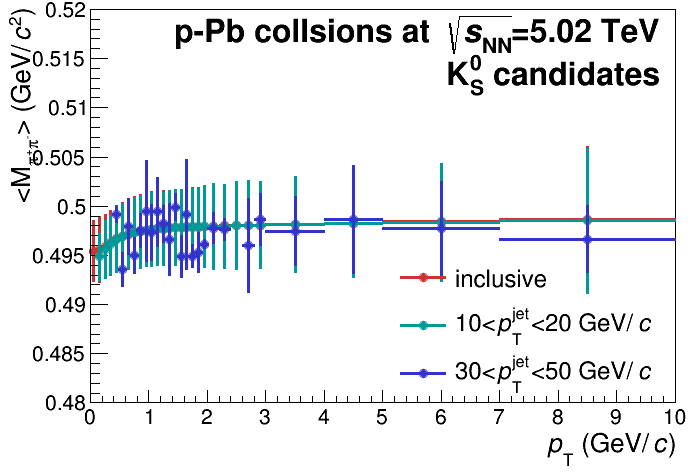
\includegraphics[width=.49\textwidth]{c02/KshortInvM}
%%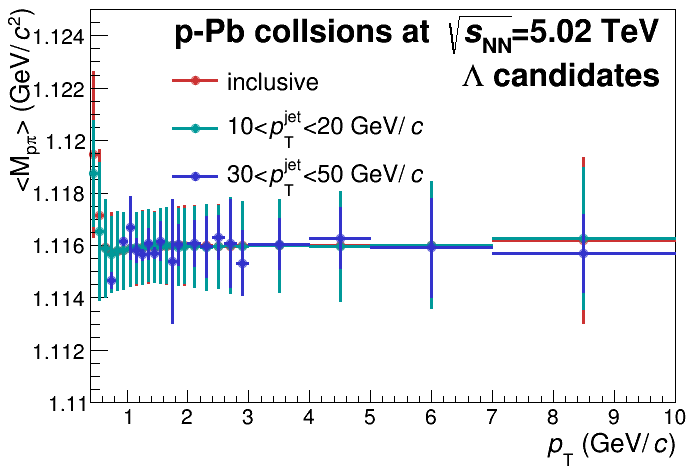
\includegraphics[width=.49\textwidth]{c02/LambdaInvM}
%%\caption{The mean and width of \Vzero\ invariant mass distribution extracted
%%         by the Gaussian fit for the inclusive $\Vzeros$ candidates
%%         and JC $\Vzero$ candidates as a function of $\pT$ in data.}
%%\label{fig:V0FitInvM}
%%\end{center}
%%\end{figure}

%%Figure~\ref{fig:V0FitInvM} shows the comparison of the mean and width of \Vzero\ invariant mass distribution extracted by the Gaussian fit for the inclusive \Vzeros\ candidates and JC \Vzero\ candidates as a function of $\pT$ in data.
%%The mean and width in the $\Vzero$ invariant mass distributions for the inclusive \Vzeros\ and JC \Vzeros\ are compatible within statistical uncertainties.
%%To avoid statistic fluctuations found in high-\pT\ jet selection, the number of JC \Vzeros is extracted using the mean and width obtained in the inclusive $\Vzero$ invariant mass distribution.

%%Given the track selection and the matching procedure the efficiency for finding a \Vzero\ within a jet is a product of single particle \Vzero\ efficiency and jet finding efficiency.

%%%%%%%%%%%%%%%%%%%%%%%%%%%%%%%%%%%%%%%%%%%%%%%%%%%%%%%%%%%%%%%%%%

%%\subsection{\Vzero\ particles from the underlying event}
%%\label{sec:V0UE}

In order to extract the \Vzero\ yield in the underlying event (not associated to the hard scatterings tagged by the charged jets considered in this analysis) several estimators have been investigated:
\begin{itemize}
  \item the so-called {\it outside cone} (OC) selection: the \Vzero\ particles that were not matched to any jet considered in the analysis within events containing a jet such that $\Delta R_{\Vzero-{\rm jet}} > R_{\rm cut}$;
  \item the {\it perpendicular cones} (PC) selection: the \Vzero\ particles found at azimuthal angles larger than $R_{\rm cut}$: $\Delta \varphi > R_{\rm cut}$, where $\Delta \varphi= \varphi^{\rm jet} - \varphi^{\Vzero}$  %%\ask{(say the value)}
  \item the {\it non-jet events } (NJ) selection: the \Vzero particles found in events that do not contain a jet with $\ptjet>5~\gevc$.
\end{itemize}

In practice, a useful quantity for performing the subtraction of the non-jet contribution of the \Vzero\ particles is their density per unit area 
\begin{equation}
\rho^{\Vzero}(\pt) = N^{\Vzero}(\pt) / A^{\Vzero},
\label{eq:defv0rho}
\end{equation}
where $N^{\Vzero}$ is the number of particles and $A^{\Vzero}$ is the acceptance in pseudo-rapidity and azimuthal angle. Consequently, the number of the UE \Vzero\ particles within a jet can be calculated as $N=\rho^{\Vzero} \Ajet$ for each estimator separately. Note, in this analysis we consider the jet area $\Ajet = \pi R^2$. Depending on the background estimator several estimators for the density of \Vzero\ particles within jets (JC) can be considered such that $\rhovzero_{\mathrm{JC}} = \rhovzero_{\mathrm{JC, raw}} - \rhovzero_{\mathrm{UE}}$, where $\mathrm{UE}$ can be any of the OC, PC, NJ. In this analysis we choose PC as the reference and use OC and NJ for the systematic uncertainty estimation.

%%%%%%%%%%%%%%%%%%%%%%%%%%%%%%%%%%%%%%%%%%%%%%%%%%%%%%%%%%%%%%%%%%
%%\subsection{\Vzero\ reconstruction efficiency}
\subsection{Corrections for \Vzero\ reconstruction and feed-down}
\label{sec:c05V0EffiMC}

The reconstruction efficiencies of \Vzero\ particles were estimated using DPMJET Monte Carlo generator \cite{Roesler:2000he} with the same cuts as in the data except the daughter track PID with ${\rm d}E/{\rm d}x$ in TPC. 
%%Figure~\ref{fig:c05EffiIncV0s} shows the efficiency of the inclusive $\Vzeros$ as a function of $\pT$ in three event multiplicity bins. 
%%For each of the event multiplicity class the efficiency is compared to the efficiency in minimum-bias events and it is found that the efficiency of inclusive $\Vzeros$ is independent on the event multiplicity.
%%\end{figure}
%%\end{center}
%%\label{fig:c05EffiIncV0s}
%%\caption{Efficiency of inclusive $\Vzeros$ as a function of $\pT$ in three event multiplicity bins with V0A centrality estimator.}
%%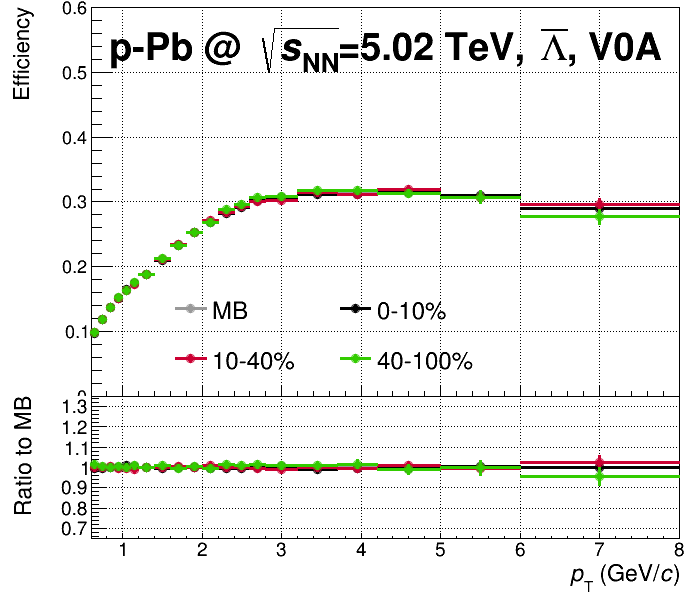
\includegraphics[width=.32\textwidth]{c02/cAntiLa_Efficiency}
%%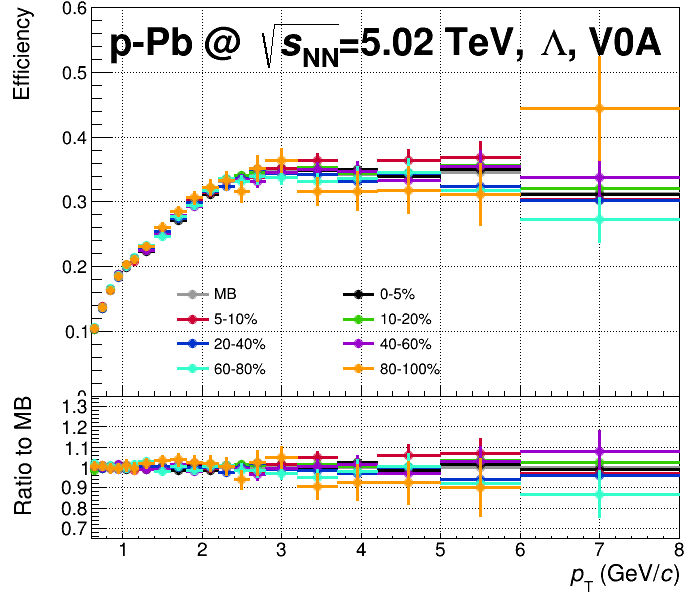
\includegraphics[width=.32\textwidth]{c02/cLambda_Efficiency}
%%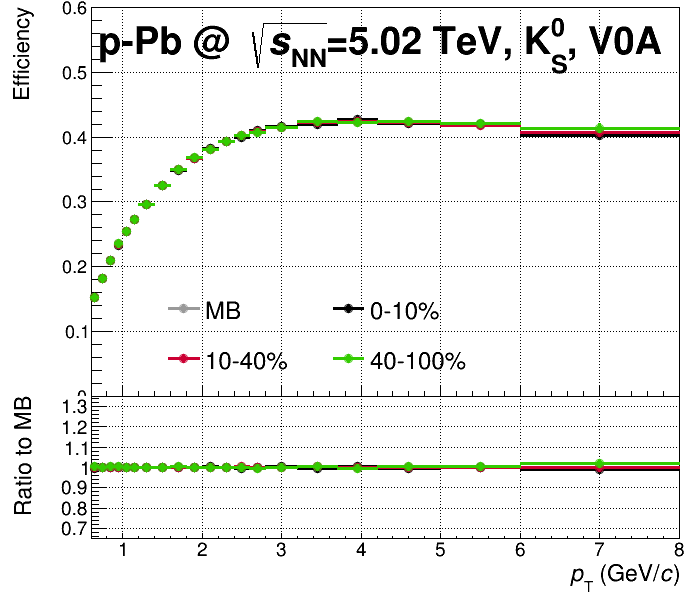
\includegraphics[width=.32\textwidth]{c02/cKshort_Efficiency}
%%\begin{center}
%%\begin{figure}[htb]

\begin{figure}[htb]
\begin{center}
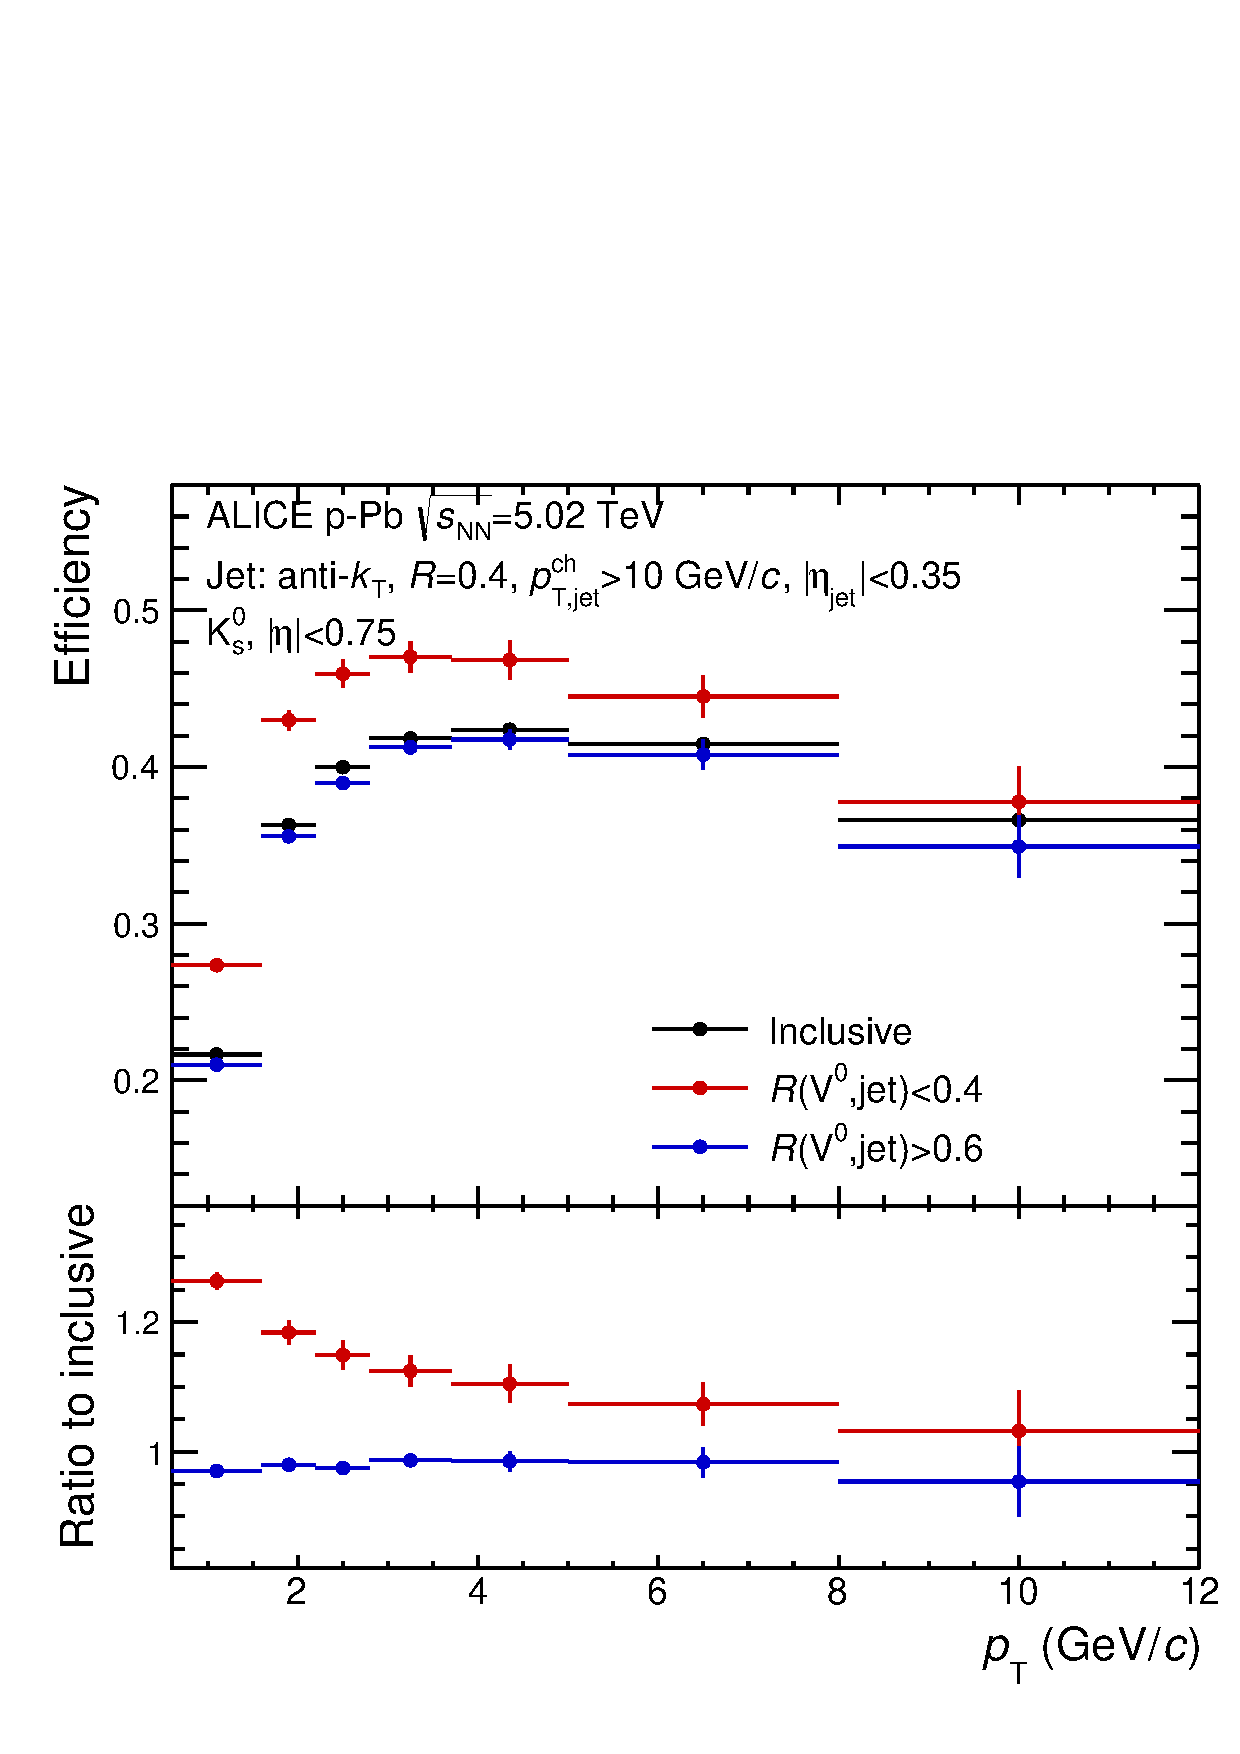
\includegraphics[width=.32\textwidth]{cEffiInJE_Kshort_JE_JR04_JC04}
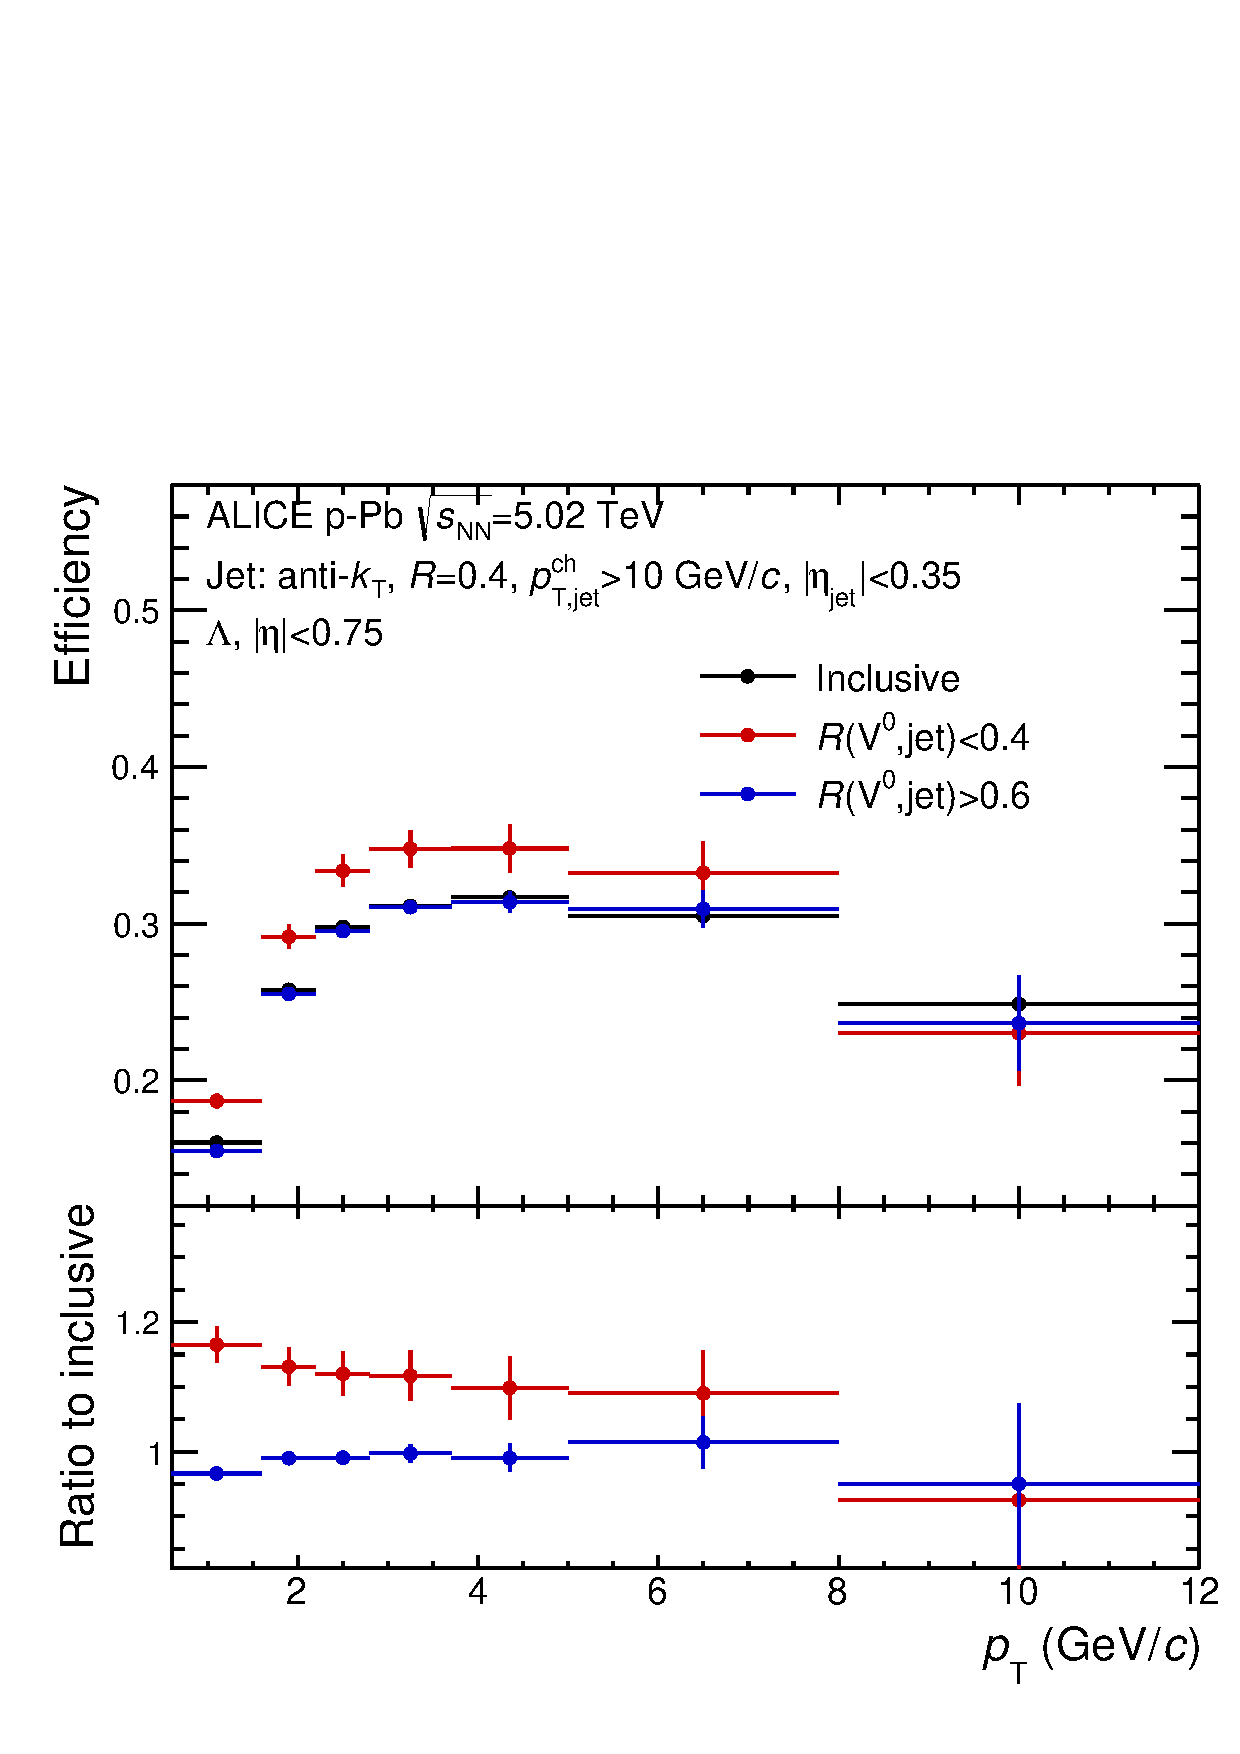
\includegraphics[width=.32\textwidth]{cEffiInJE_Lambda_JE_JR04_JC04}
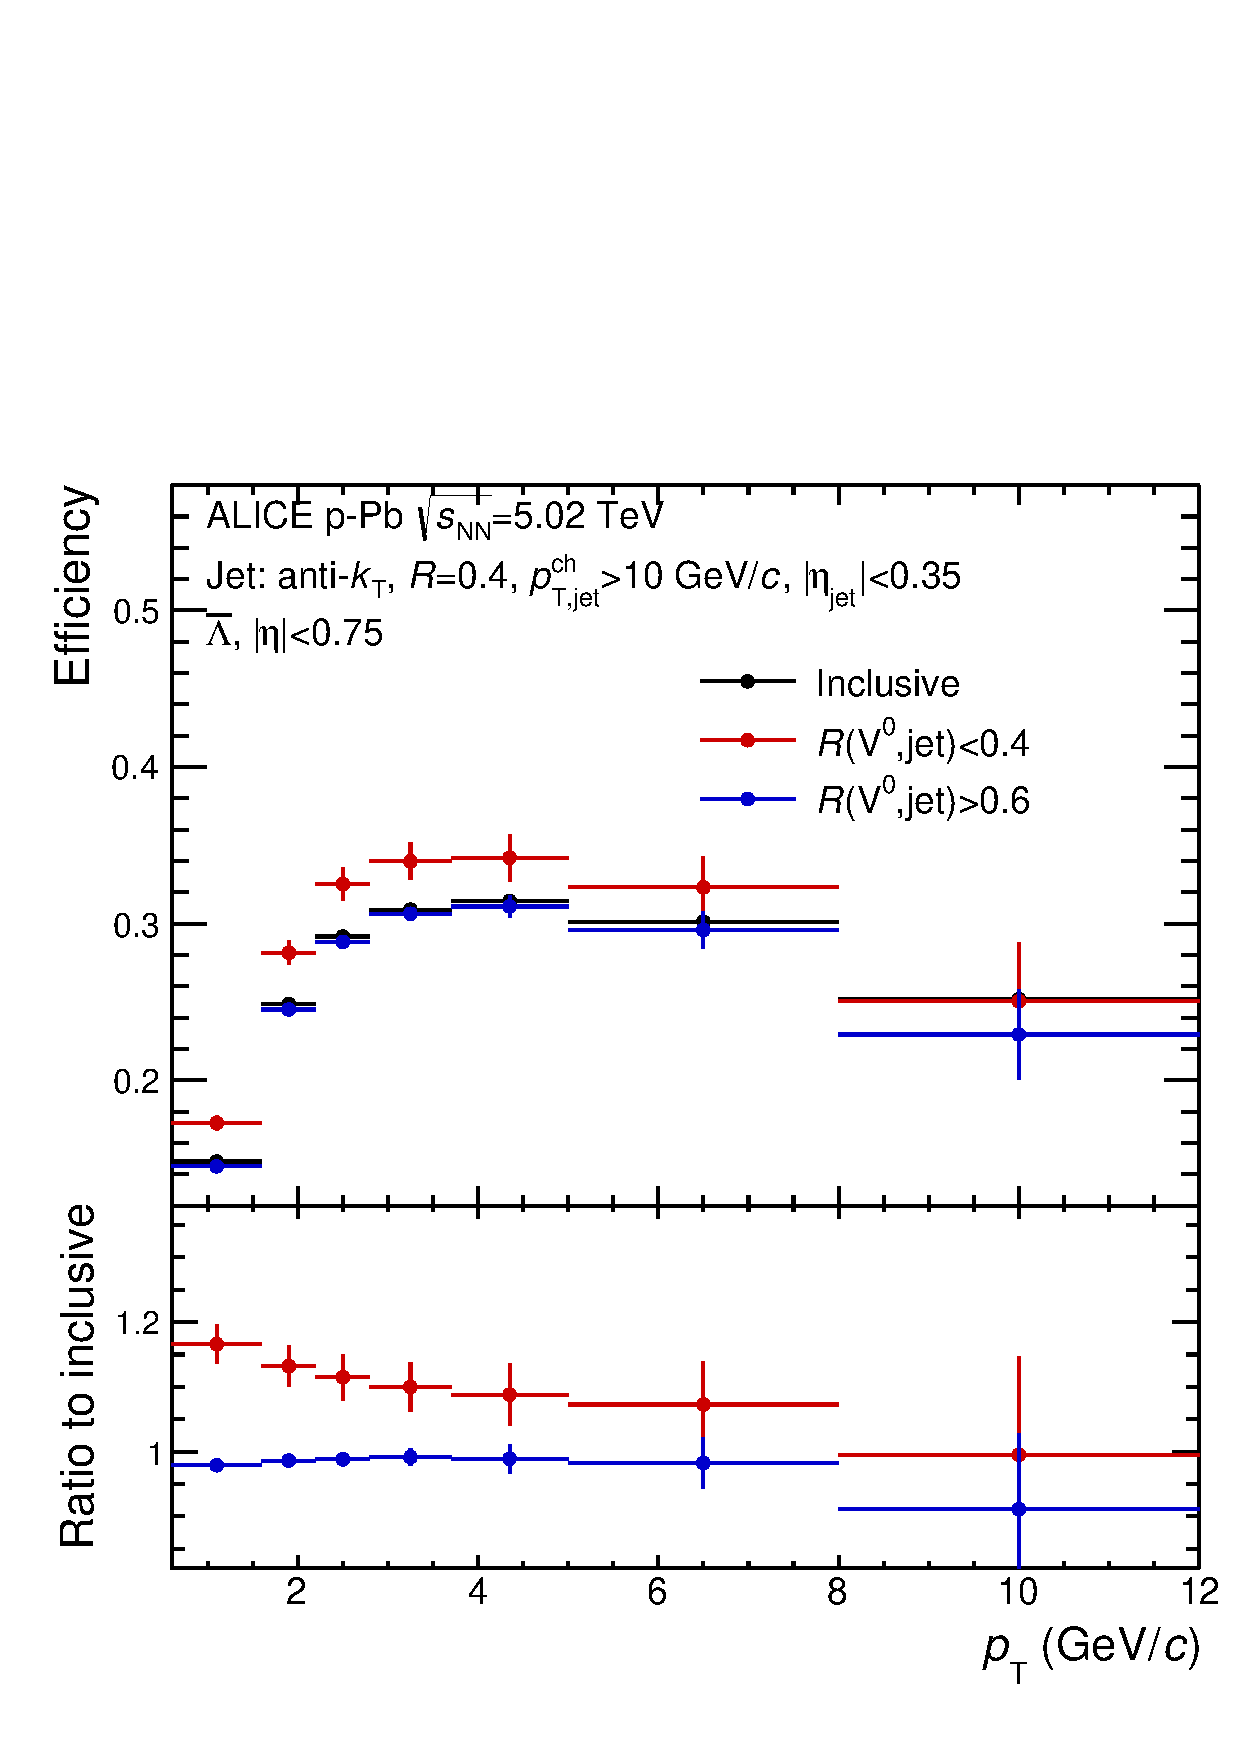
\includegraphics[width=.32\textwidth]{cEffiInJE_AntiLa_JE_JR04_JC04}
\caption{Efficiency of \Vzero\ particles in \pPb\ collisions at \sqrtsnn{5.02} for three selections: inclusive, within $\Delta R_{\Vzero-{\rm jet}} <0.4$ and $\Delta R_{\Vzero-{\rm jet}} >0.6$.}
\label{fig:c02EffiIncV0s}
\end{center}
\end{figure}

Due to differences in the experimental acceptance for \Vzero\ particles associated to jets (JC) and those extracted through the various estimators of the underlying event (OC, PC, NJ) the efficiencies of \Vzero\ particles were estimated separately for every case. Figure \ref{fig:c02EffiIncV0s} shows the inclusive reconstruction efficiency for $\Vzero$ particles and the efficiency in the events containing a jet for two selections of distance $R$ from the main jet axis. The efficiency for events containing a jet varies with $R$ and for every selection of $R$ the efficiencies were evaluated separately. \ask{Jana: add info how does the efficiency varies with R...}

%%%%%%%%%%%%%%%%%%%%%%%%%%%%%%%%%%%%%%%%%%%%%%%%%%%%%%%%%%%%%%%%%%
%%\subsection{Feed-down subtraction for \lda\ and \alda}

The \pt\ differential yields of \lda\ and \alda\ reconstructed for each selection (JC and UE selections) where corrected for the feed-down from $\Xi$ decays. 
%%The correction was applied before the efficiency corrections. 
The $\Xi$ production in jets (JC) was estimated based on measurements of the multi-strange baryons and their decays at high-\pt\ performed in \pp\ collisions \cite{Abelev:2012jp} and extrapolated to the lower \pt\ using PYTHIA event generator and full detector simulations.
The applied correction is about 15\% and largely independent of the \lda\ and \alda\ momentum. \ask{check numbers}
Conversely, \lda\ yields were not corrected for the feed-down from $\Omega^{-}$ baryons nor for the feed-down from non-weak decays of $\Xi^{0}$ and $\Xi(1385)$ family as these contributions are neglibible as compared to the systematic uncertainties of the present measurement.

%%%%%%%%%%%%%%%%%%%%%%%%%%%%%%%%%%%%%%%%%%%%%%%%%%%%%%%%%%%%%%%%%%

\subsection{Systematic uncertainties}
\label{sec:uncertainties}

%%\subsection{Uncertainties in \Vzero\ particle reconstruction}

The main sources in the \Vzero\ particle reconstruction are the level of knowledge of detector materials (resulting in a 4\% uncertainty), track selections (up to 5\%) and the feed-down correction for the \lda\ (5\%), while topological selections contribute 2-4\% depending on transverse momentum. 
These systematic uncertainties are summarized in Table \ref{tab:v0syst} and presented in Fig. \ref{fig:systUncert}.

\begin{table}[t]
\centering 
\begin{tabular*}{\linewidth}{@{\extracolsep{\fill}}lccc}
\hline
&&&\\[-0.7em]
 & \kzero\ & \multicolumn{2}{c}{\lmb(\almb)}\\[0.3em]
\hline
&&&\\[-0.7em]
Proper lifetime & 2\% & \multicolumn{2}{c}{2\%} \\[0.3em]
Material budget & 4\% & \multicolumn{2}{c}{4\%} \\[0.3em]
Track selection  & 4\% & \multicolumn{2}{c}{4\%} \\[0.3em]
TPC PID & 1\% & \multicolumn{2}{c}{1\%} \\[0.3em]
%Multiplicity & \multirow{2}{*}{2\%} & \multicolumn{2}{c}{\multirow{2}{*}{2\%}} \\
%dependence & & \\[0.3em]
\hline
\hline
&&&\\[-0.7em]
\pt\ (\gevc)  &  & $<$ 3.7 & $>$ 3.7\\[0.3em]
\hline
&&&\\[-0.7em]
Feed-down  &  & \multirow{2}{*}{5\%} & \multirow{2}{*}{7\%}\\
correction & & &\\[0.3em]
    \hline
    \hline
    &&&\\[-0.7em]
\pt\ (\gevc)  &  & $<$ 3.7 & $>$ 3.7\\[0.3em]
    \hline
    &&&\\[-0.7em]
    Total & 6.5\% & 8\% & 9.5\% \\[0.3em]
\hline
\end{tabular*}
\caption{Main sources of systematic uncertainty for the \kzero\ and \lmb(\almb).} \label{tab:v0syst}
\end{table}

\begin{figure}[htbp]
	\centering
	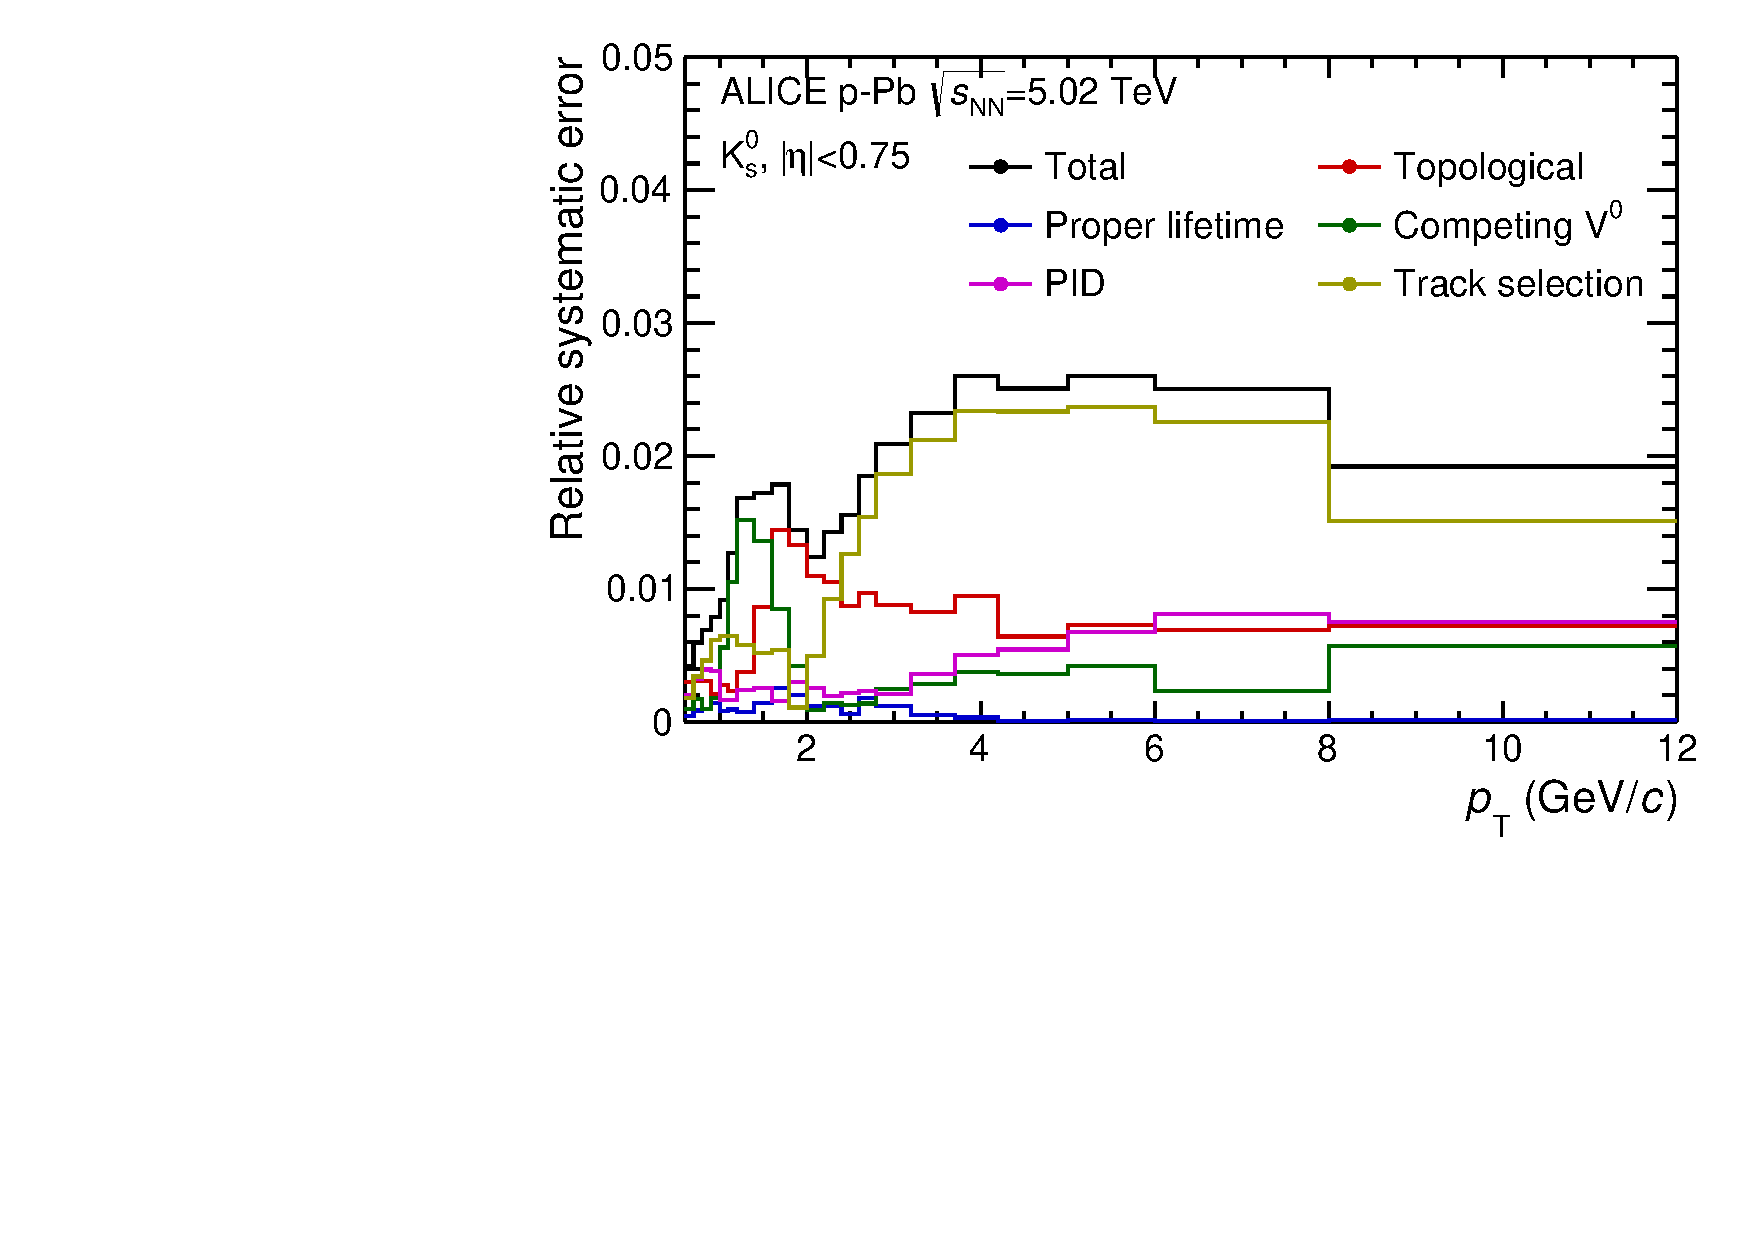
\includegraphics[width=0.32\textwidth]{cSystIncl_Kshort}
	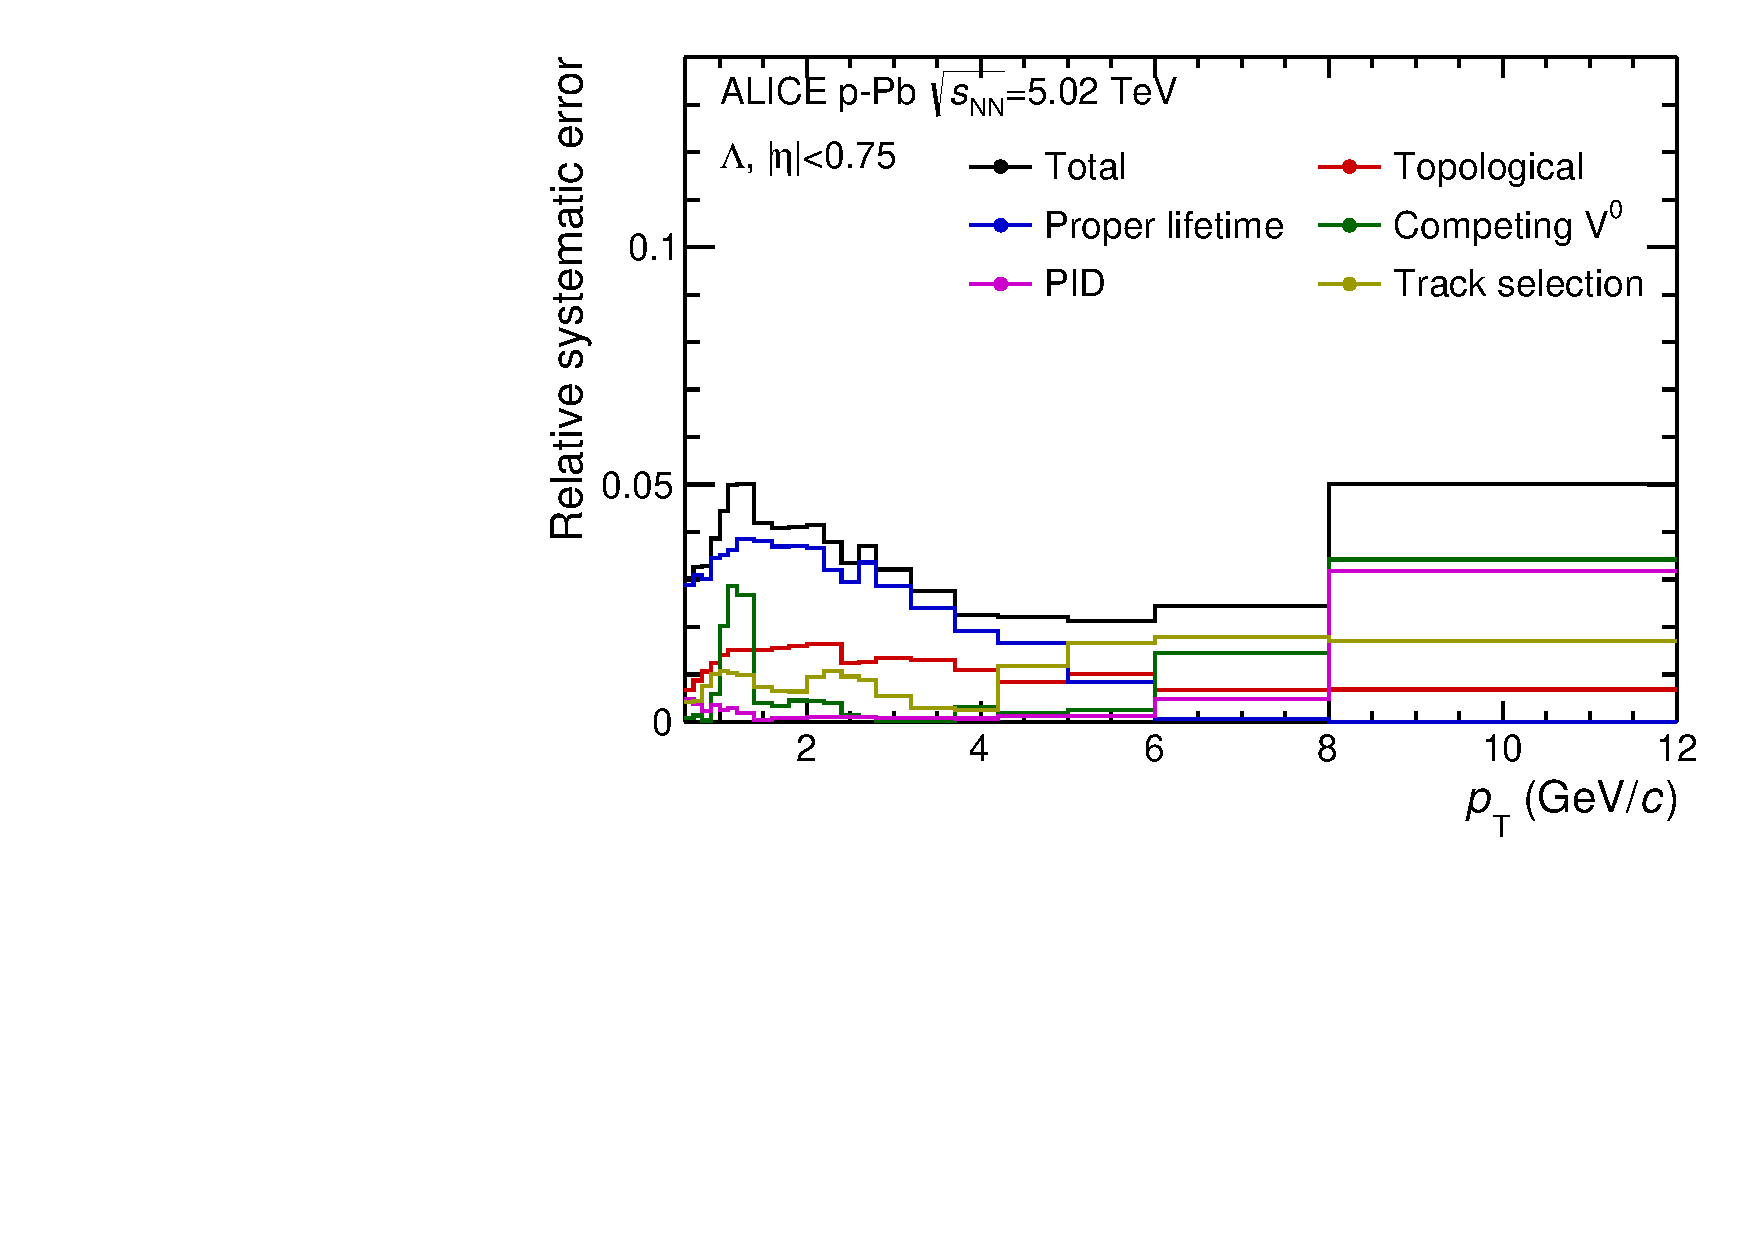
\includegraphics[width=0.32\textwidth]{cSystIncl_Lambda}
	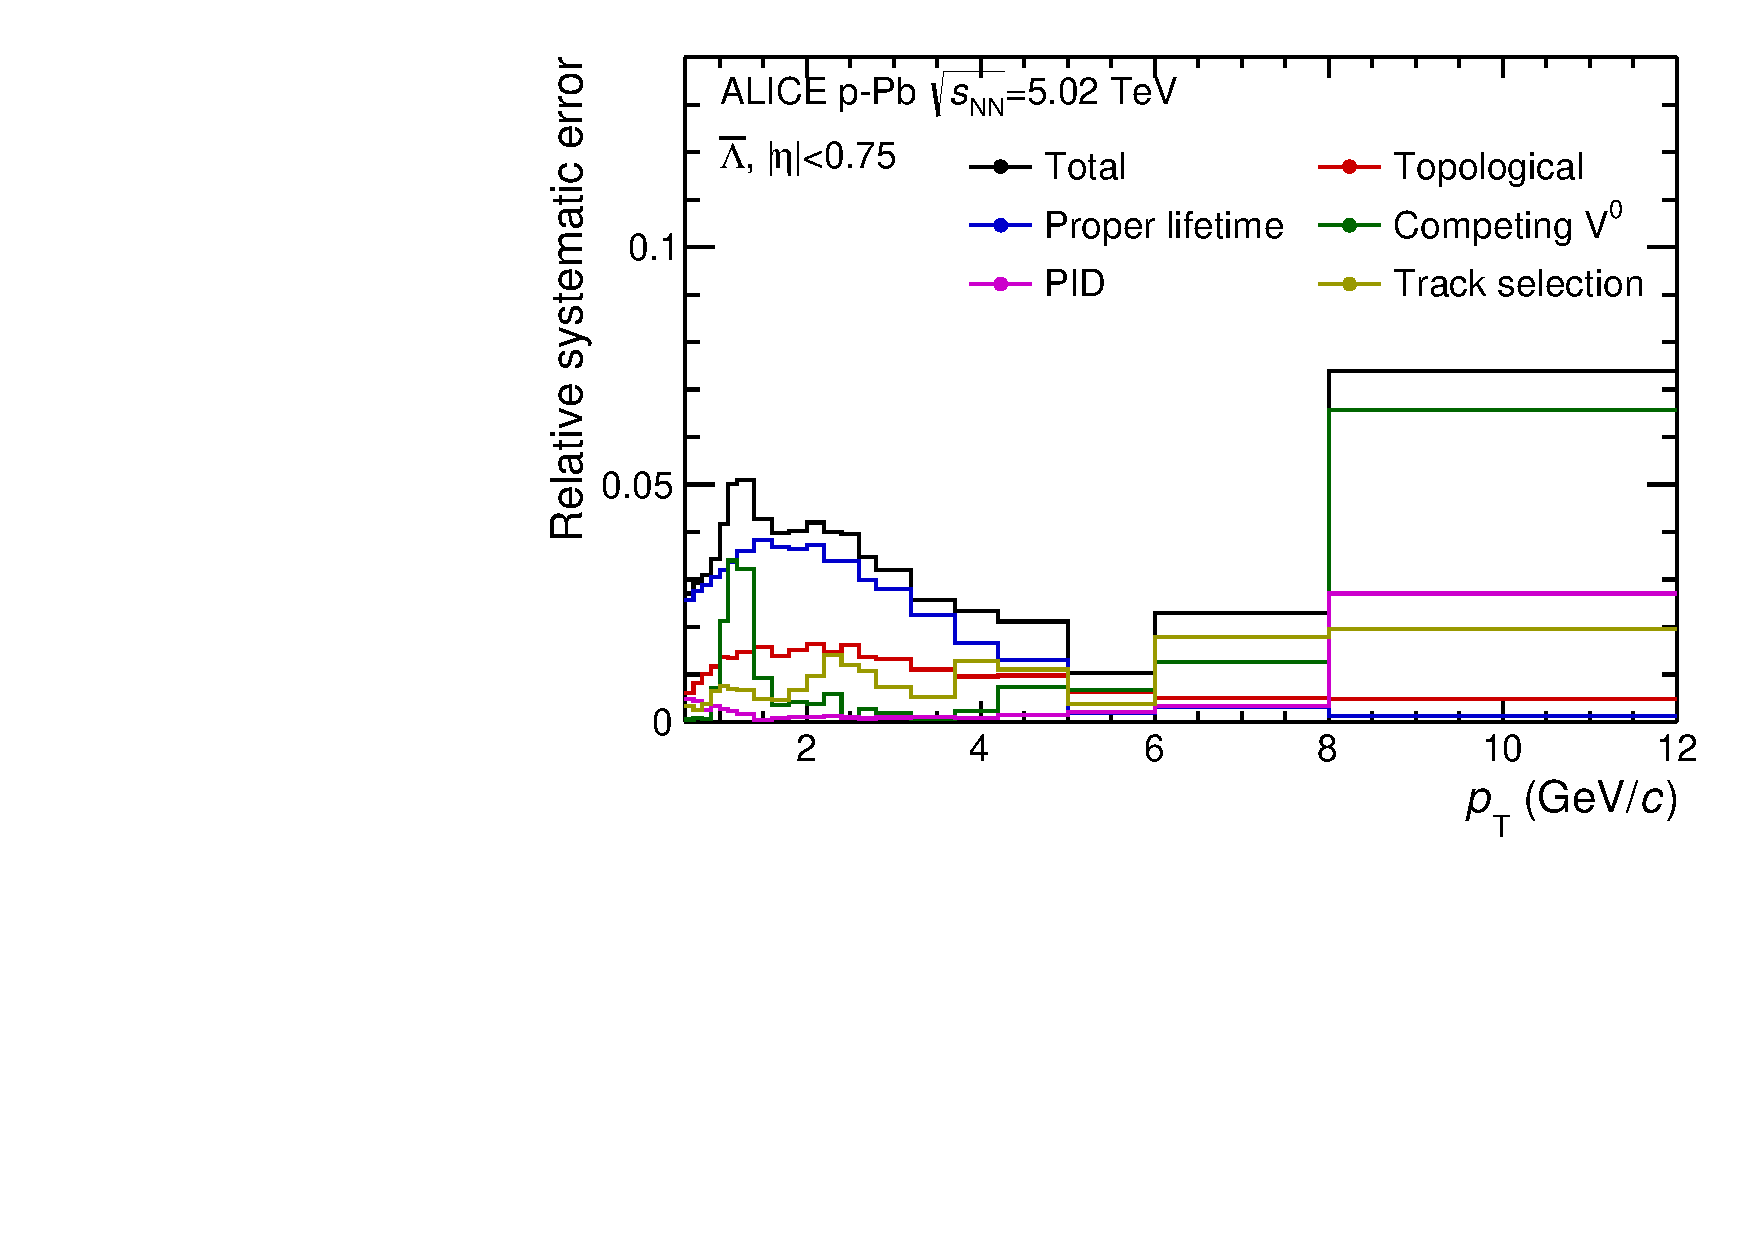
\includegraphics[width=0.32\textwidth]{cSystIncl_AntiLa}
	\caption{Systematic uncertainties on \Vzero\ particle spectrum (left: \ks, center: \lda, right: \alda) as a function of their transverse momentum (see text and Tab. \ref{tab:v0syst} for details).}
	\label{fig:systUncert}
\end{figure}

%%%%%%%%%%%%%%%%%%%%%%%%%%%%%%%%%%%%%%%%%%%%%%%%%%%%%%%%%%%%%%%%%%%%%

%%\subsubsection{Uncertainty in UE \Vzero\ estimation}

%%\ask{sections below need more quant. and phrasing to be checked; also add a summary figure as a function \pt}

The systematic uncertainties on the particle spectra and their ratios originating from the sources discussed below are added in quadrature. 
\ask{Jana: We should also note how are the systematic uncertainties propagated to the lambda/K0S ratio.}
Two main sources of uncertainties originating from the mis-association of \Vzero particles with UE were considered:
\begin{itemize}
\item the \Vzero\ particle was found outside the selected jet and classified as UE particle; however, it may have originated from a physical jet outside the fiducial acceptance for jets considered in the analysis and/or from a {\it true} low-\pt\ jet, below the considered thresholds;
\item the \Vzero\ particle originates from a true high-\pt\ jet; however, due to the finite detector efficiency the jet has not been reconstructed above the considered \pt\ threshold.
\end{itemize}

The uncertainty on the UE \Vzero\ density has been estimated using the two variations of the UE estimators: the {\it outside cone} (OC) and the {\it non-jet events} (NJ).
The OC and the NJ estimators encapsulate the maximum deviation in the yield of UE particles and the difference of the reconstructed \Vzero\ yields in OC and NJ has been included as the additional systematic uncertainties on the density of particles within the jets (JC). 
The uncerainty is largest for low-momenta particles ($< 2~\gevc$) reaching up to 30\% but drops rapidly with \pt\ to negligible values at $6~\gevc$. \ask{check numbers}.

%%%%%%%%%%%%%%%%%%%%%%%%%%%%%%%%%%%%%%%%%%%%%%%%%%%%%%%%%%%%%%%%%%%%%

%%\subsubsection{Jet reconstruction and jet selection}

The systematic uncertainty originating from the selection of the jet \pt\ were estimated by repeating the analysis with jet \pt\ varied around the chosen thresholds of 10 and 20~\gevc\ by 2~\gevc. 
This variation accounts for jet resolution due to detector effects and the fluctuations of the event background density as reported in \cite{Adam:2015hoa}. 
For jets $\ptch>10~\gevc$ At low momenta ($\ptvzero<2\gevc$) it reaches up to 10\% and 20\% for jets of $\ptch>20~\gevc$. The uncertainty remains almost a constant 5\% for $\ptvzero > 2~\gevc$ independently of the $\ptch$. \ask{check numbers}

\begin{figure}[htbp]
	\centering
	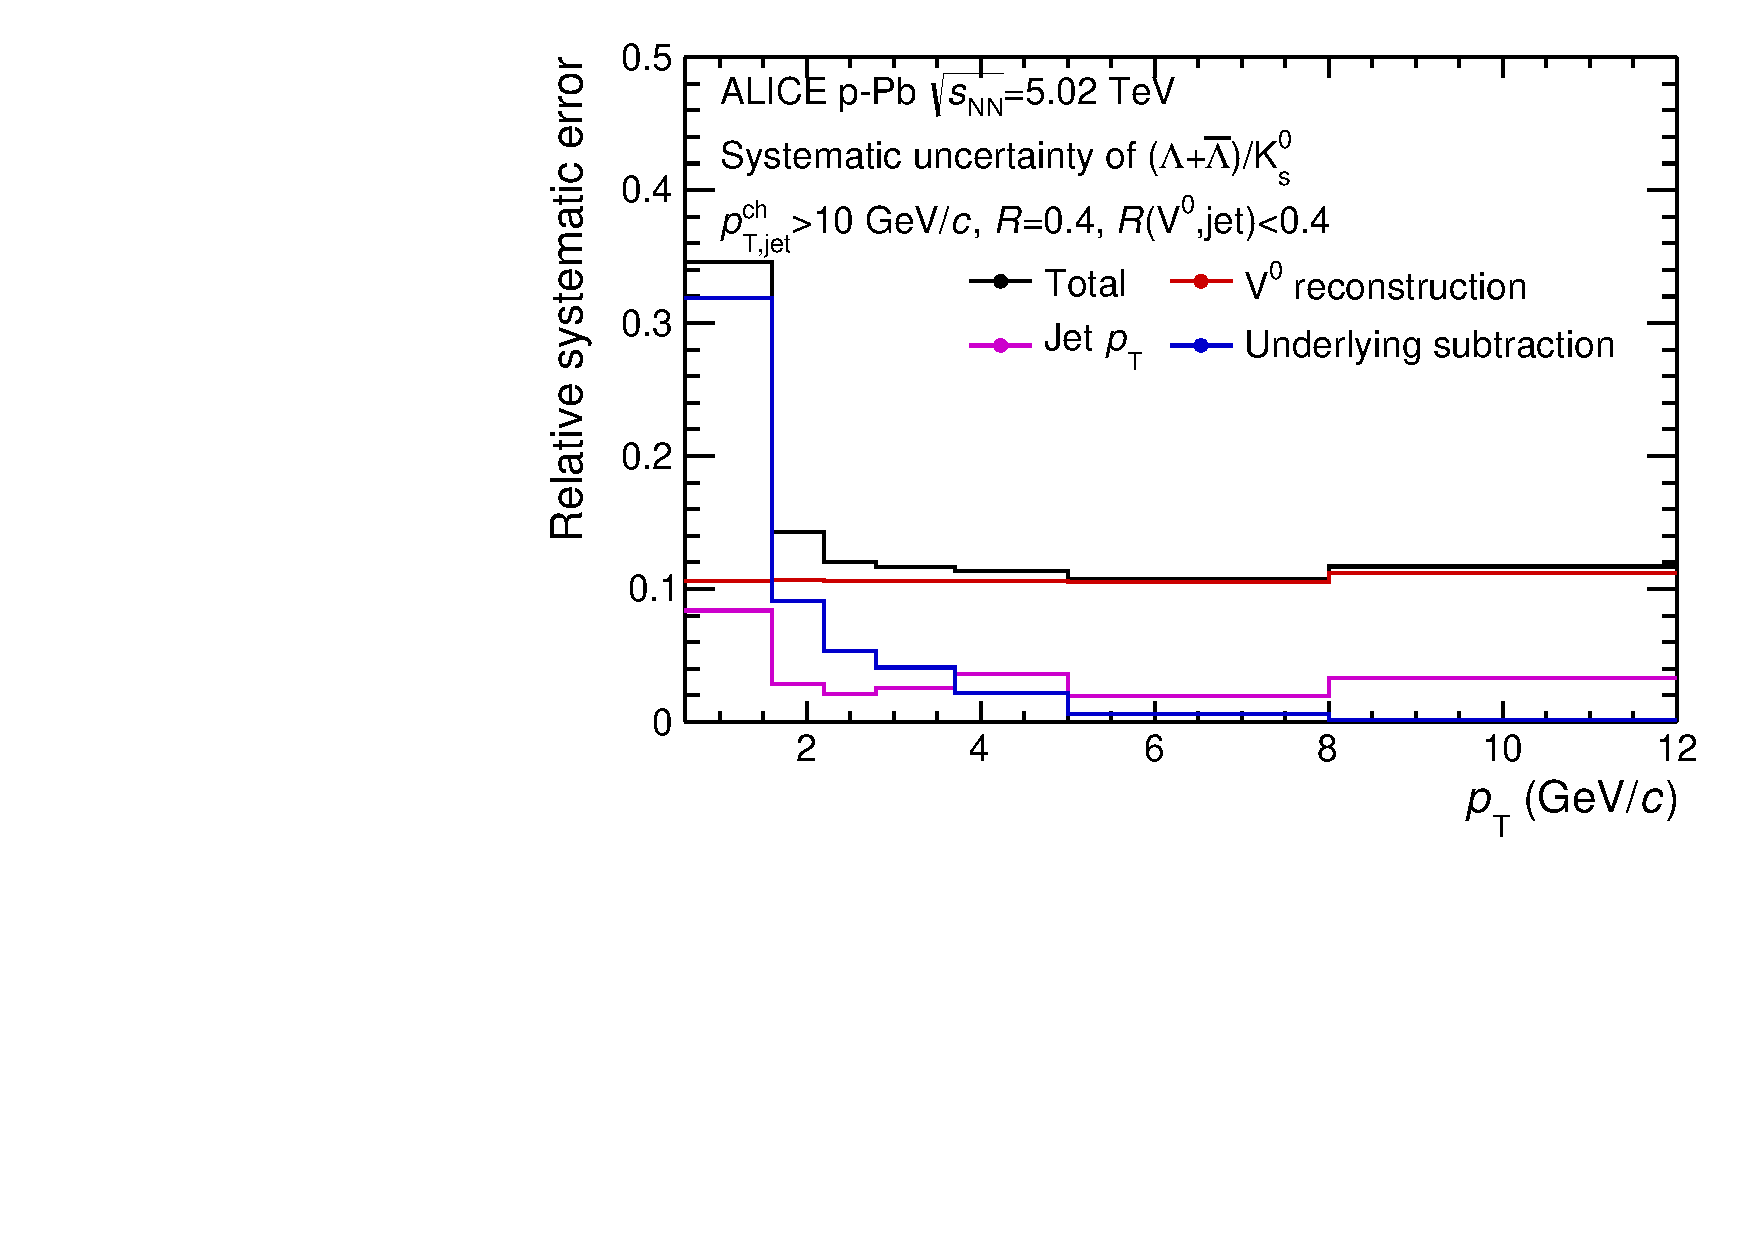
\includegraphics[width=0.47\textwidth]{cSystInJE_RatioV_Ptj10}
	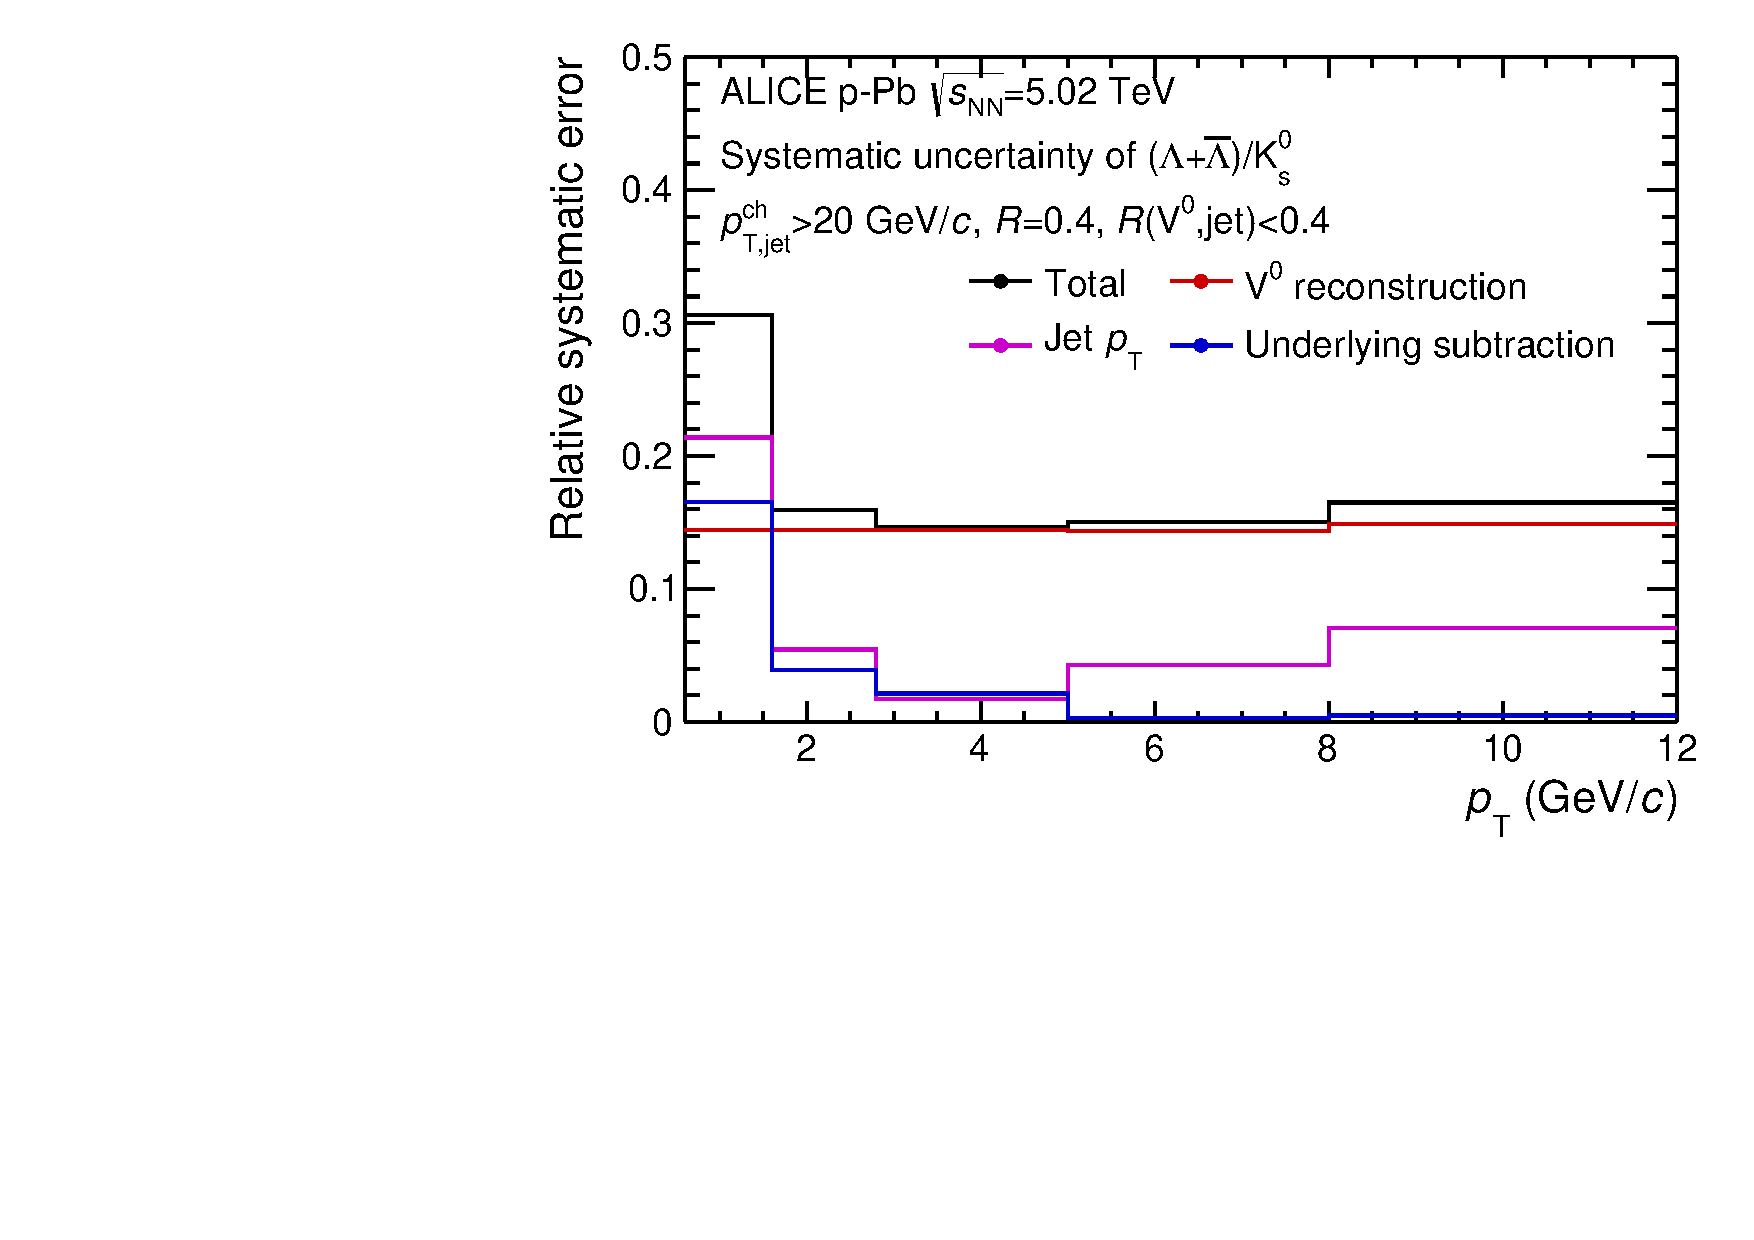
\includegraphics[width=0.47\textwidth]{cSystInJE_RatioV_Ptj20}
	\caption{Relative systematic uncertainty on the ratio of \lda\ and \ks\ spectrum within $R=0.4$ anti-\kt\ jets for $\ptch>10~\gevc$ (left) and $\ptch>20~\gevc$ (right) as a function of particle \pt. Three contributions to the total uncertainty are shown: uncertainty on \vzero\ reconstruction, uncertainty on the underlying event subtraction, and uncertainty on the jet momentum scale and momentum resolution. }
	\label{fig:systUncertRatio}
\end{figure}

Figure \ref{fig:systUncertRatio} shows the relative systematic uncertainties on the \lda/\ks\ ratio reconstructed within $R=0.4$ jets with $\ptch > 10~\gevc$ and $\ptch > 20~\gevc$ as a function of particles \pt. 
For the $\ptch > 20~\gevc$ the total uncertainty is about 16\% and is largely independent of particle \pt\ with the largest contribution of 14\% originating from the uncertainty on \Vzero\ reconstruction.

%%\ask{what about jet finding efficiency? - what is the rec. efficiency and how it varies with the fragmentation model? => estmated from the jets where no jets was found... the UE subtraction -> jets where only particles produced are \lda\ and/or \ks\ ?}

%%%%%%%%%%%%%%%%%%%%%%%%%%%%%%%%%%%%%%%%%%%%%%%%%%%%%%%%%%%%%%%%%%%%%

\section{Results}
\label{sec:Results}

\subsection{\pt\ dependent strange particle densities}

The fully corrected densities of \ks\ and the sum of \lda\ and \alda\ particles associated to a hard scattering tagged by a jet are shown in Fig. \ref{fig:rhov0}. 
The per jet density within the jet cone (JC) is compared to the density for inclusive particles (without association to jets) and to the density in the perpendicular cones (PC).
In the case of inclusive particles the distribution is normalized to the product of the total number of events and the acceptance of the \vzero\ particles in a single event (full azimuth and $|\eta|<0.75$). 
As expected, for both \ks\ and \lda\ particles the density within jets is much harder as the high-\pt\ particles originate from jets. 
The density in the PC selection is qualitatively similar to the inclusive distribution showing strong \pt\ dependence. 
Both, the inclusive and the PC distributions show a rapid decrease with \pt\ reaching values more than an order of magnitude lower than the JC density for particle \pt\ exceeding $4~\gevc$.
This is consistent with an expectation that the high-\pt\ particles originate from jet fragmentation.

\begin{figure}[htbp]
	\centering
	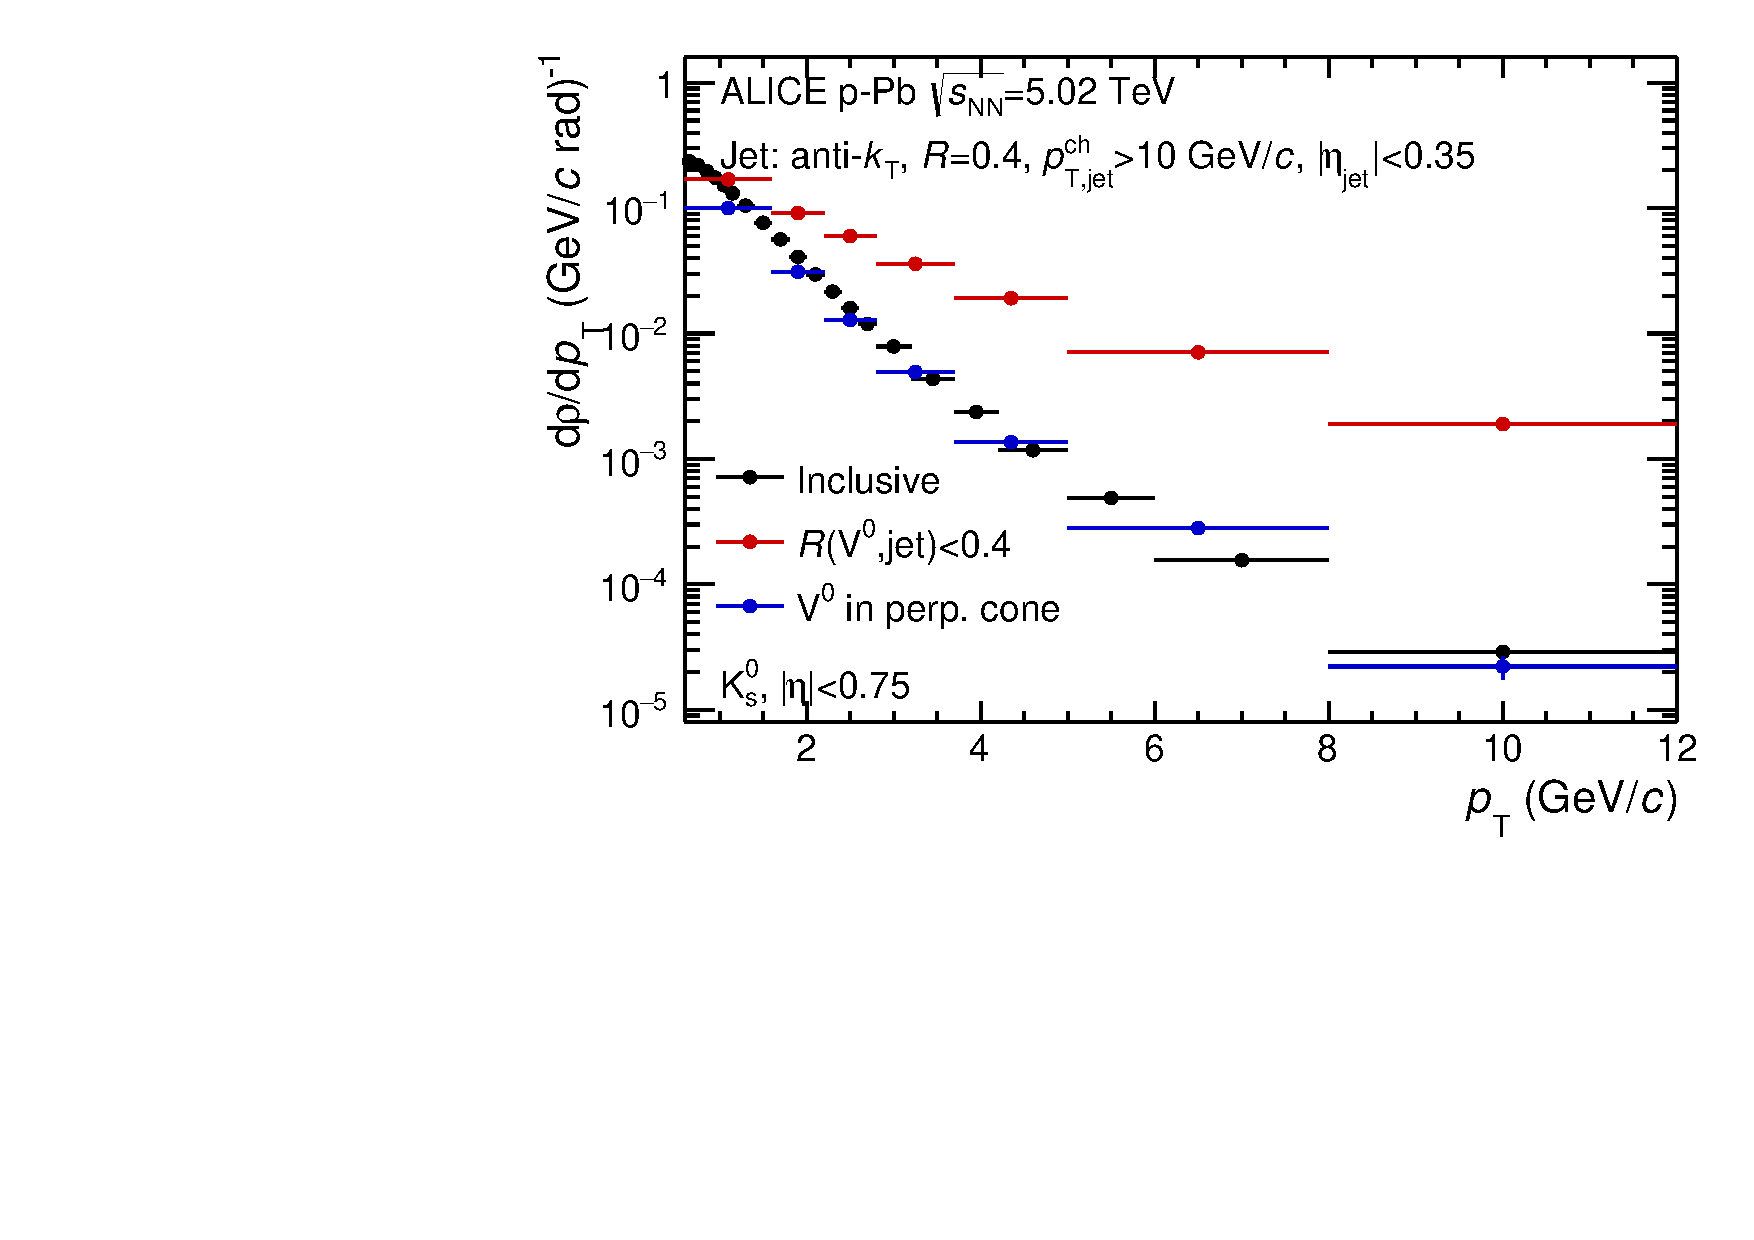
\includegraphics[width=0.47\textwidth]{cRho_Kshort_JE_JR04_JC04}
	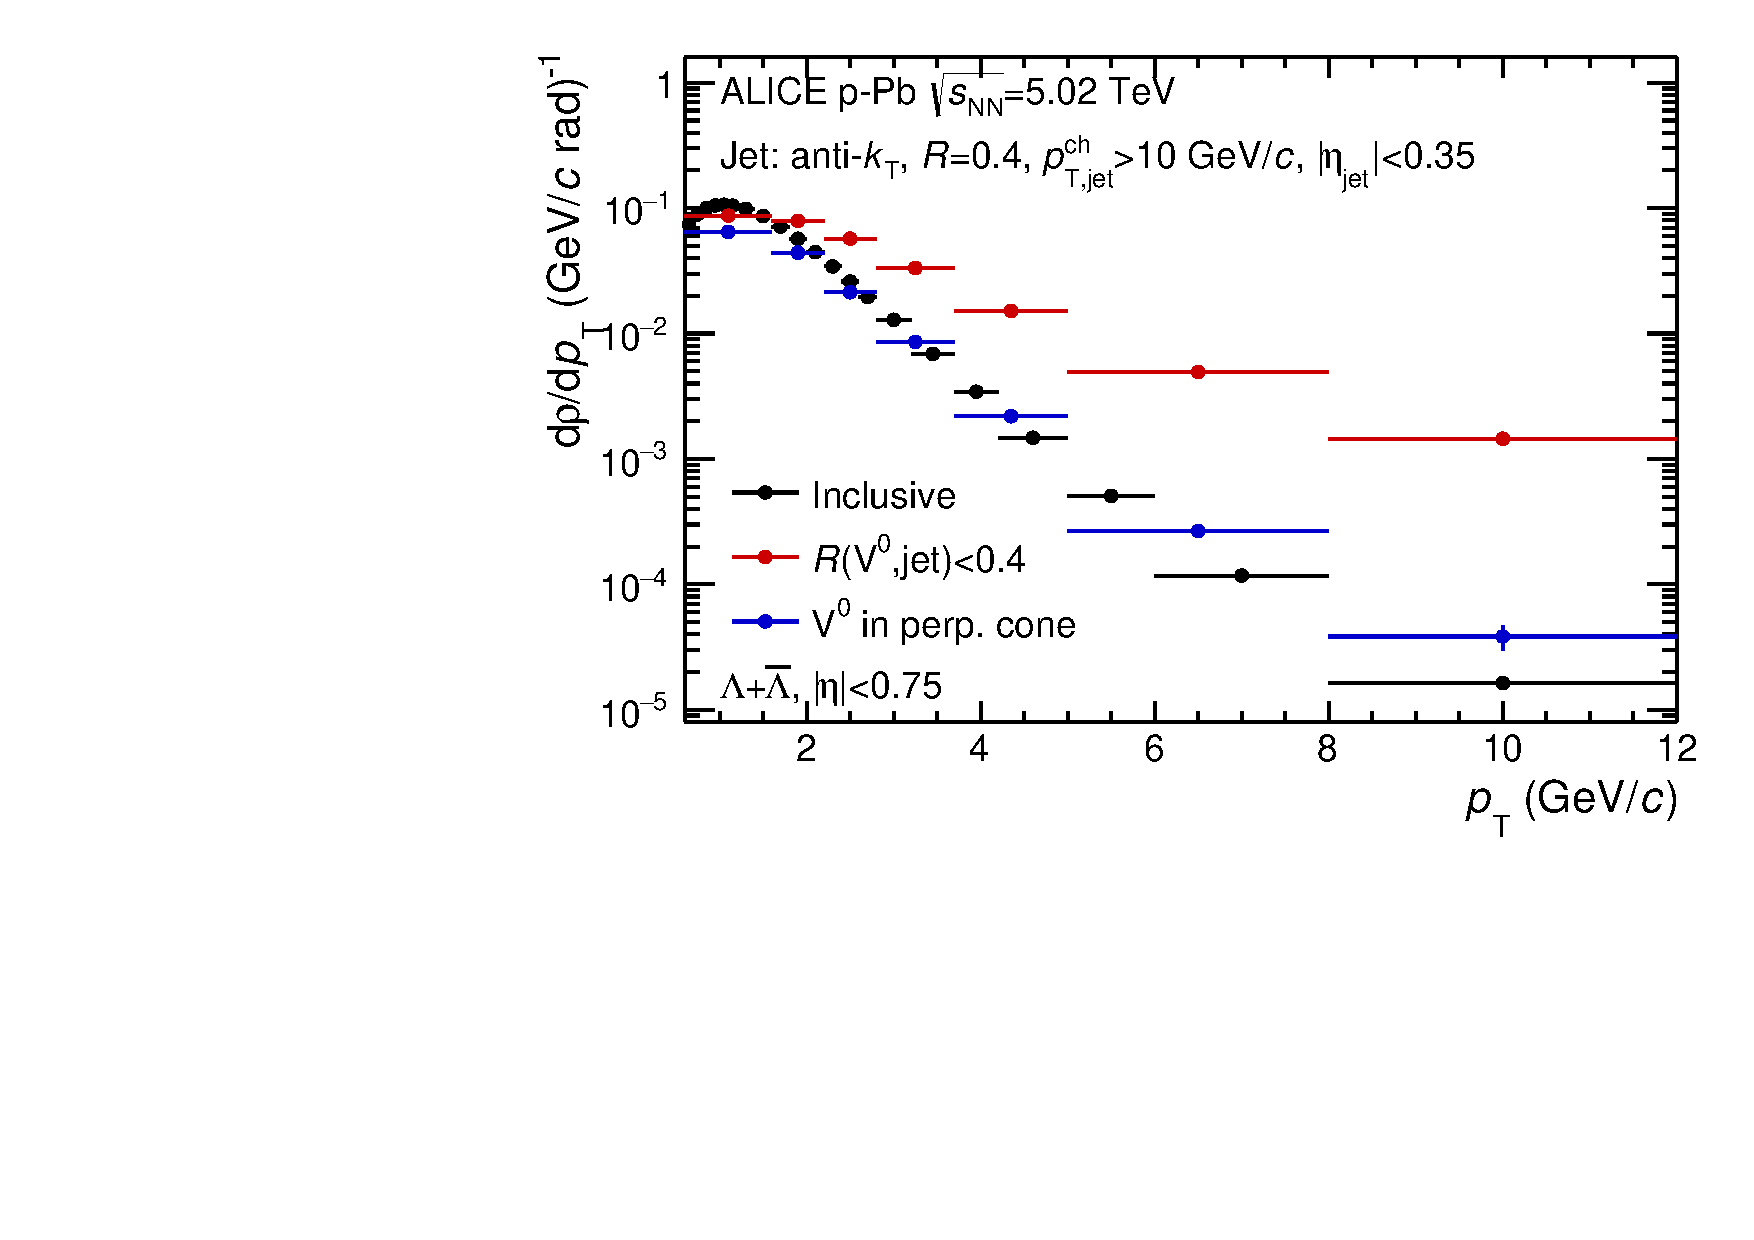
\includegraphics[width=0.47\textwidth]{cRho_Lambda_JE_JR04_JC04}
	\caption{Differential density of particles \drhodpt\ (see Eq. \ref{eq:defv0rho}) in p-Pb collisions at \sqrtsnn{5.02} for \ks\ (left), and the sum of \lda\ and \alda\ (right). The density is shown for three selections: inclusive particles from minimum bias events, particles within a anti-\kt\ jet ($\ptch>10~\gevc$) with $R=0.4$ and the perpendicular cones (PC) in events containing the jet.}
	\label{fig:rhov0}
\end{figure}

\subsection{\lda\ks\ ratios}
%the ratio is not sensitive to the jet resolution parameter $R$ 

Ratios of \lda\ and \ks\ yields can be obtained by dividing the normalized density distributions. In the following the sum of \lda\ and \alda\ densities is divided by twice the density of \ks. \ask{MP/Jana: average / K or sum / (2xK)?}
Moreover, as no significant difference was found for different jet resolution parameters $R$ the results are presented as the average of results obtained with $R$ of 0.2, 0.3, and 0.4. 
Figure \ref{fig:LKR} shows the ratio for the JC selection as a function of the distance from the jet axis \rvzerojet\ without subtracting the UE backgrounds. 
The ratio is shown for three momentum bins: the low-\pt\ ($0.6 <\pt <1.8~\gevc$), inermediate \pt\ ($2.2 < \pt < 3.7~\gevc$), and the high-\pt\ ($4.2 < \pt < 12~\gevc$). 
The ratio as a function of \rvzerojet\ at low-\pt\ remains approximately constant at about $0.2$ independent of the distance to the jet axis and that is the case even at large distances of $\rvzerojet > 1.2$. 
This value is consistent with the inclusive measurements in \pPb\ collisions, but also in \pp\ and peripheral \PbPb\ collisions were effects related to the collective expansion of the system are either not-present or small \cite{Abelev:2014uua}.

Conversely the intermediate-\pt\ selection shows an increase of the ratio from about $0.3$ when evaluated close to the jet axis to values of about $0.6$ at \rvzerojet\ distances of about $0.5$.
For distances $\rvzerojet > 0.5$ the ratio remains constant.
The ratio of $0.6$ is consistent with the inclusive measurement in \pPb\ collisions \cite{Abelev:2013haa} and this \pt\ region is where the ehnanced \lda/\ks\ ratio in the inclusive measurements was found the largest.
We stress that for the results shown in Fig. \ref{fig:LKR} the UE backgrounds were not subtracted.
Therefore the evolution of the ratio as a function of the distance from the axis demonstrates how the two sources UE and jet compete.
The lack of enhancement (values consistent with \pp\ collisions) close to the jet axis indicate that the enhanced \lda/\ks\ ratio is not associated with the jets.
%%The increase to the inclusive  but rather a feature of the soft part of the event. 

In each of the momentum bins the ratio is dominated by the lower edge of the selection window due to steeply falling particle pT spectrum. 
This is especially the case for the high-\pt\ selection where the dominating component originates from \pt\ of about $4.5~\gevc$ and the \rvzerojet\ dependence at high-\pt\ is similar to intermediate \pt. The ratio at high-\pt\ accociated to jets is discussed below.

%%%%

The right panel of Fig.\ref{fig:L2Kratio} shows the ratio of \lda\ to \ks\ as a function of particle \pt\ for four selections: the inclusive particles, the particles from the PC selection, and two JC selections for jet \pt\ of $10$ and $20~\gevc$ averaged over three resolution parameters $R$ (0.2, 0.3, 0.4). 
For JC selection, prior to forming the ratio, the UE density contribution obtained with the PC selection was subtracted from the JC densities for each particle species separately.
Additionally, for the results in Fig. \ref{fig:L2Kratio} every \Vzero\ particle was required to be close to the jet axis with its distance $\rvzerojet < 0.2$.
The inclusive and the PC distributions show the enahncement at \pt\ of about $3~\gevc$. 
The ratio for the inclusive case is consistent with the measurement presented in \cite{Abelev:2013haa}.
The PC distribution above $2~\gevc$ reaches systematically higher values than the inclusive. 
The \lda-to-\ks\ ratio within jets is consistently is lower than the inclusive case and approximately independent of \pt\ beyond $2~\gevc$.
In particular, the ratio for particles associated to the jet does not show a maximum at the intermediate \pt.
This corroborates the scenario in which the enhancement of \lda/\ks\ is not present within jets.
Additionally, this conclusion holds for both, 10\gevc but also higher \pt\ ($20~\gevc$) jets.

\begin{figure}[htbp]
	\centering
	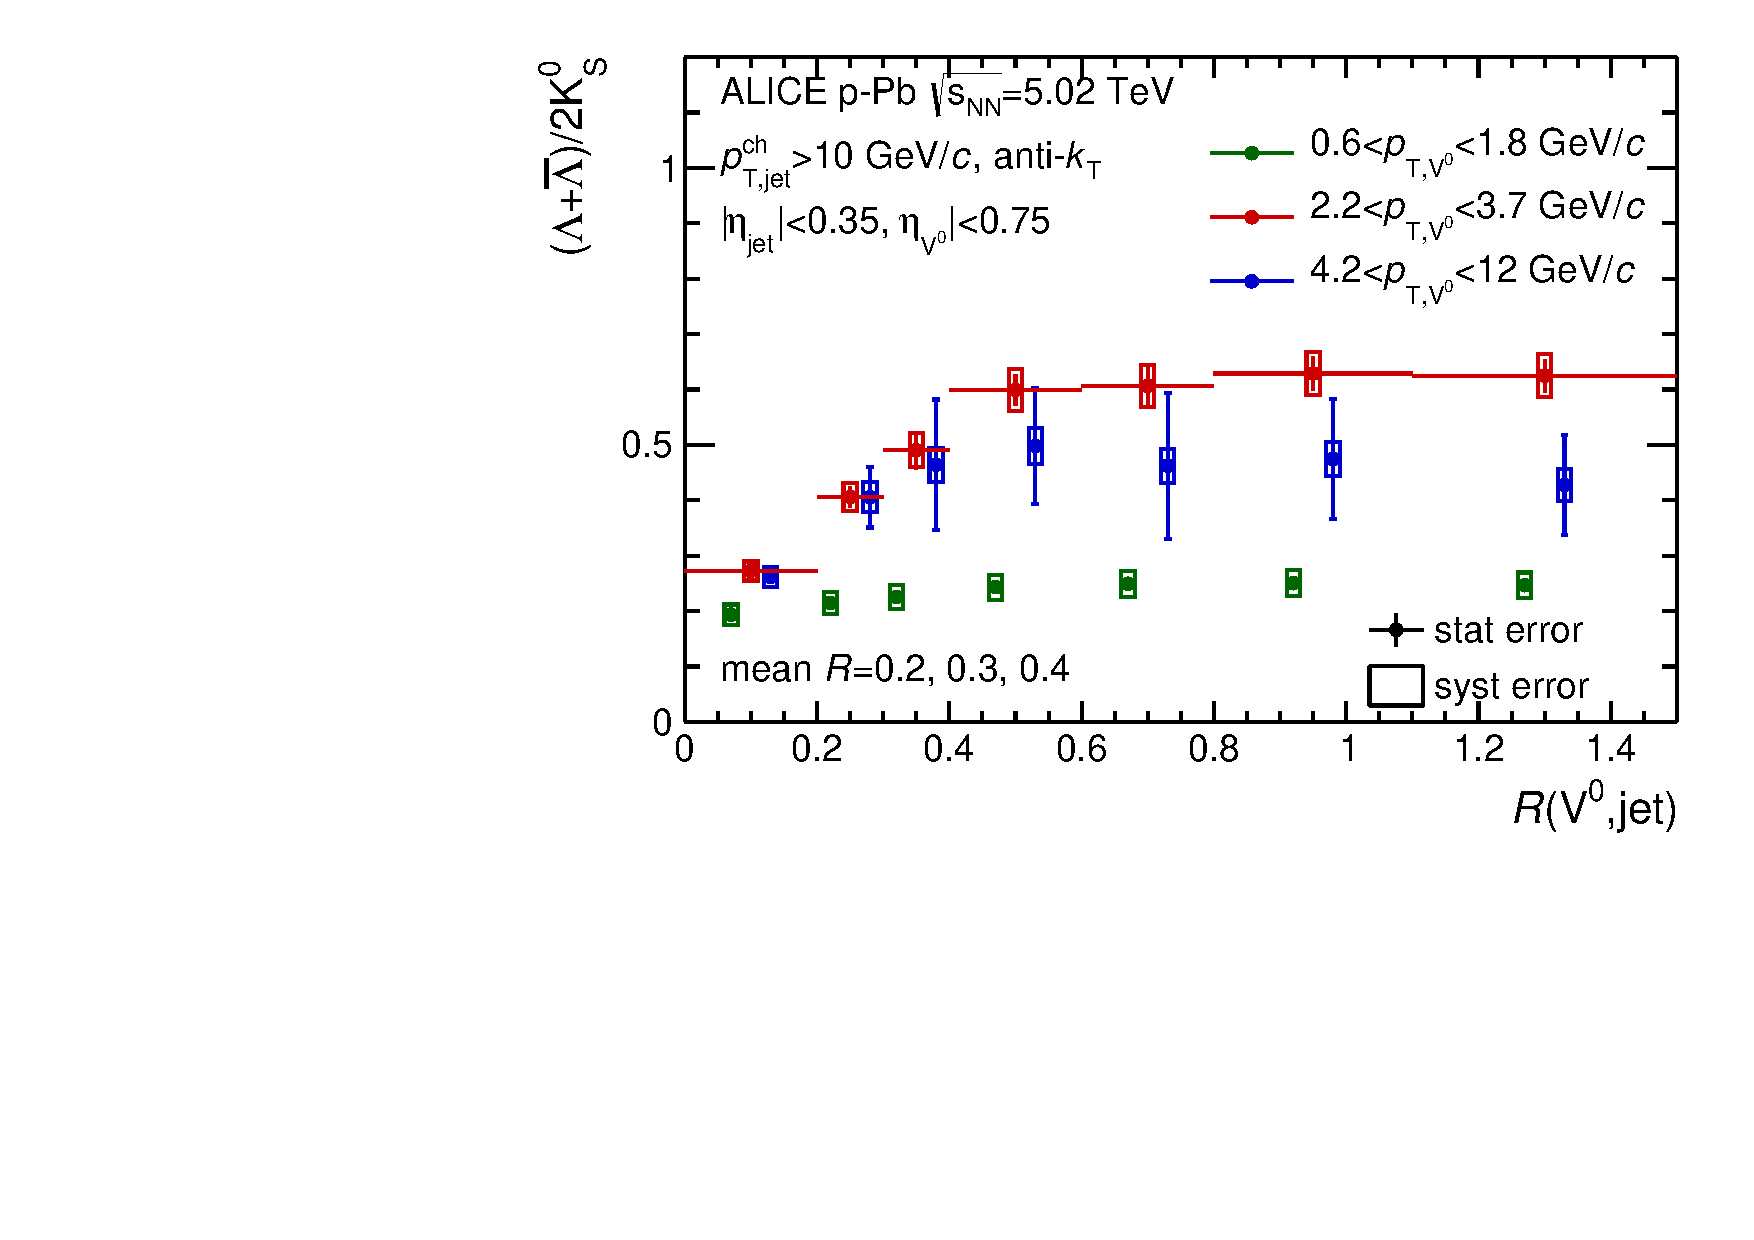
\includegraphics[width=0.47\textwidth]{cRatioV_VJ_Mean_PtJ10}
	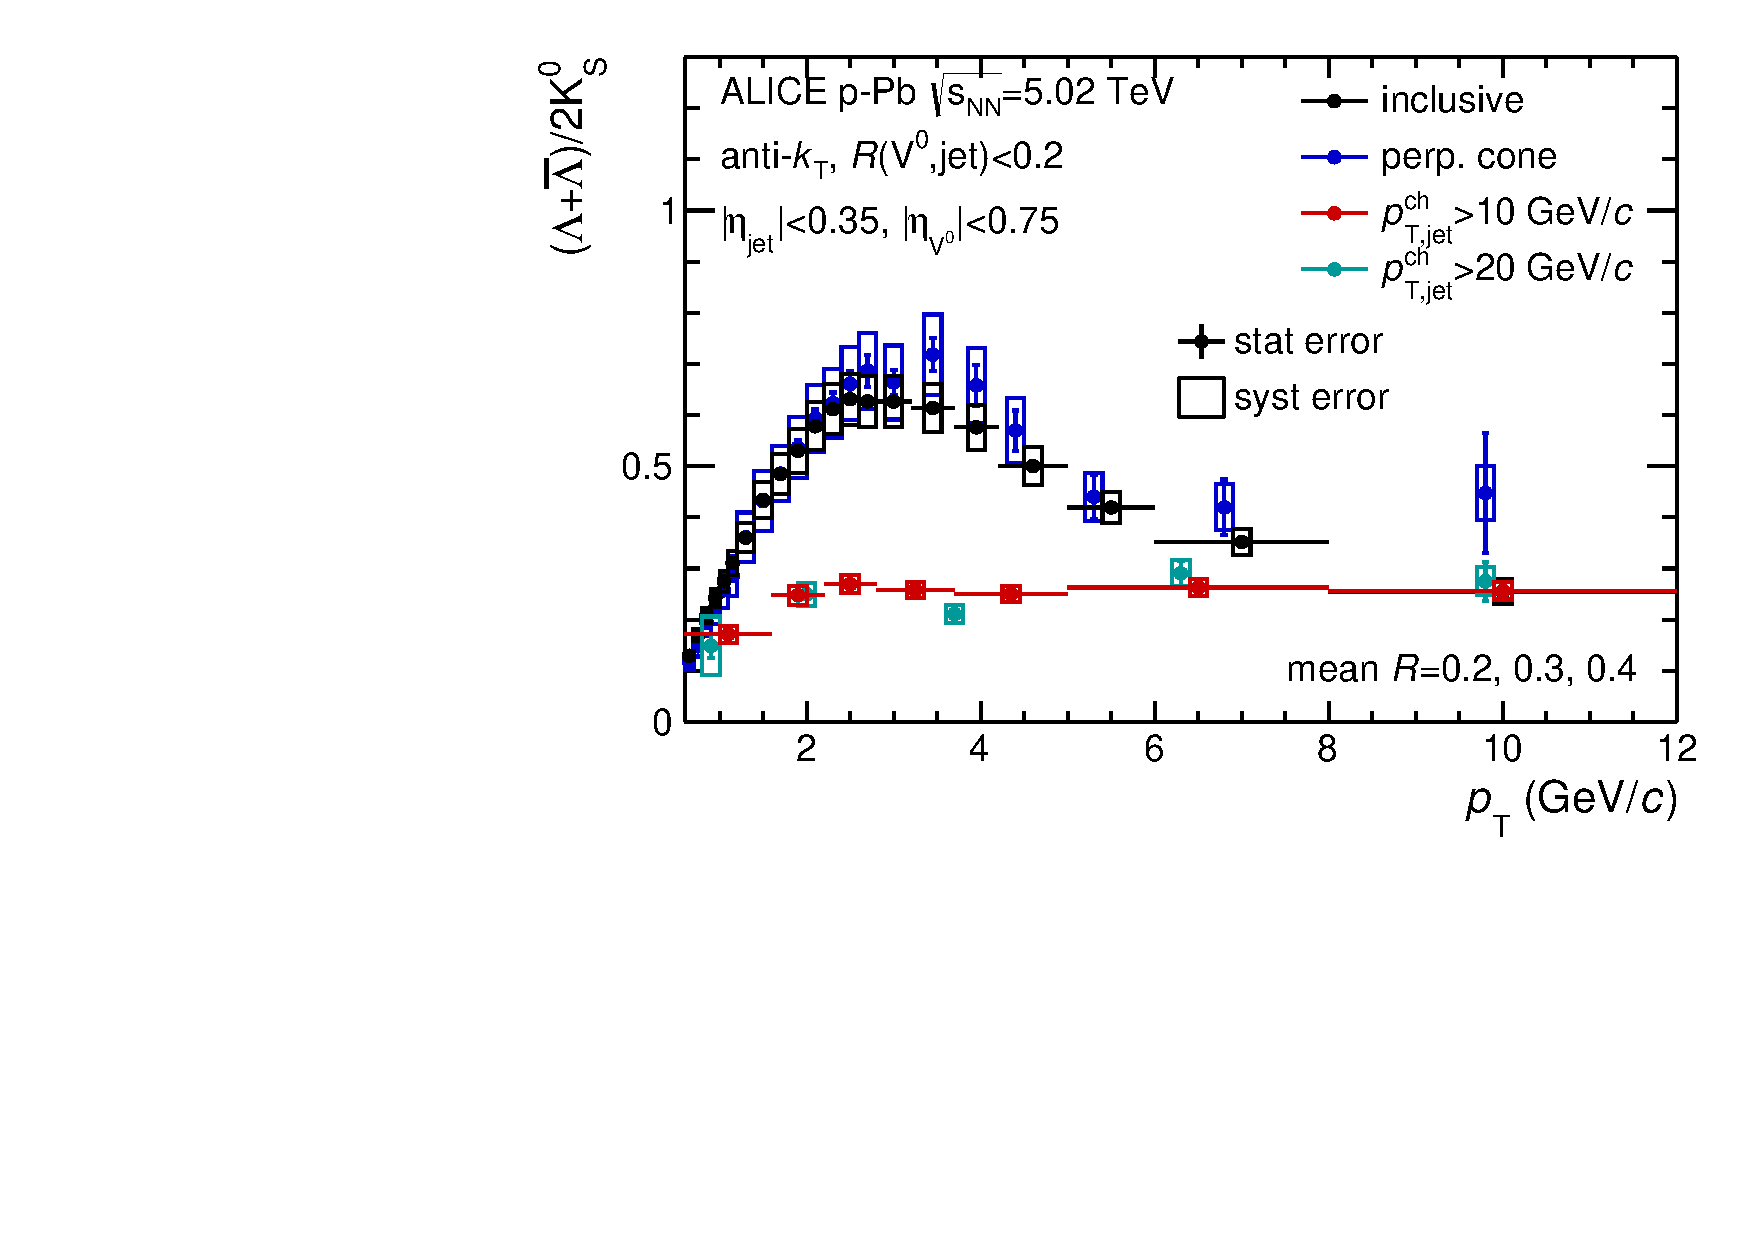
\includegraphics[width=0.47\textwidth]{cL2K_Pt_Mean_PtJE}
	\caption{\lda/\ks\ ratio in p-Pb collisions at \sqrtsnn{5.02} as a function of $\Delta R_{\Vzero-{\rm jet}}$ for three different \Vzero-particle \pt\ selections associated with charged jets with $\ptch>10~\gevc$ (left) and as a function of \Vzero-particle \pt\ associated with charged jets with pT $\ptch>10~\gevc$ and $20~\gevc$ together with that in inclusive and PC distribution (right). For more details see legend.}
	\label{fig:L2Kratio}
	\label{fig:LKR}
\end{figure}

\ask{MP: figures and the text should either use $\Delta R_{\Vzero-{\rm jet}}$ or $R_{\Vzero-{\rm jet}}$ - check were applicable.}

\ask{the following is to be reworked or removed all together - it is a comment and not altering any of the conclusions:}
Selecting hard scatterings according to the jet energy carried exclusively by the primary charged particles induces biases and inefficiencies on the jet spectrum.
The bias is related to the probabilistic process of fragmentation and hadronization.
This analysis will not tag parton showers that fragmented into a configuration of hadrons that did resulted in producing a 10 \gev\ charged particle jet with a given $R$.
Therefore, there can be cases of \Vzero\ particles that originated from a parton of a hard scattering but were not associated to a charged particle jet. 
Using PYTHIA simulations we found that the most probable \pt\ of the full jet energy is larger by about 40\%. 
Moreover, since the daughters of the \Vzero\ particles are not included in the jet energy calculation there are cases of jets containig \Vzero\ particles but not included in this analysis. 
However, the right panel of Fig. \ref{fig:L2Kratio} shows that the inclusive \lda/\ks\ ratio at high-\pt\ is fully consistent with the ratio from particles associated to jets in this analysis.

%%%%%%%%%%%%%%%%%%%%%%%%%%%%%%%%%%%%%%%%%%%%%%%%%%%%%%%%%%%%%%%%%%%%%

\section{Summary}

In conclusion, the enhancement in the ratio of inlcusive \lda, \alda\ and \ks\ found in the \pPb\ and \PbPb\ collisions is not present for particles associated to a hard scattering. 

\ask{from the PbPb paper:
The agreement between collision systems suggests that the relative fragmentation into \lda\ and \ks\ hadrons at high pT, even in central collisions, is vacuum-like and not modified by the medium.
}

As such enhancement has been linked to the interplay of radial flow and parton recombination at intermediate-\pt\ its absence within the jet cone demonstrates that these effects are confined to a soft particle production and do not modify jet composition. 

%\begin{enumerate}
%	\item spectra harder in jets
%	\item L/K ratio: a) different than inclusive or OC/PC/NJ/inclusive - no peak; b) consistent with vacuum within uncertainties -> UE radial flow; jets do not flow
%	%%\item mean \pt -> hint softening of jet fragments in most central collisions? - tension with 2.b
%	\item constraint on the soft-hard parton recombination (?)
%\end{enumerate}

               %%%%%%%%%%% put the body of the article here
%
%

%%%%% acknowledgements
\newenvironment{acknowledgement}{\relax}{\relax}
\begin{acknowledgement}
\section*{Acknowledgements}
%The ALICE Collaboration would like to thank all its engineers and technicians
for their invaluable contributions to the construction of the experiment and
the CERN accelerator teams for the outstanding performance of the LHC complex.
%
The ALICE Collaboration gratefully acknowledges the resources and support
provided by all Grid centres and the Worldwide LHC Computing Grid (WLCG)
collaboration.
%
The ALICE Collaboration acknowledges the following funding agencies for
their support in building and running the ALICE detector:
%
State Committee of Science,  World Federation of Scientists (WFS)
and Swiss Fonds Kidagan, Armenia,
%
Conselho Nacional de Desenvolvimento Cient\'{\i}fico e Tecnol\'{o}gico (CNPq),
Financiadora de Estudos e Projetos (FINEP),
Funda\c{c}\~{a}o de Amparo \`{a} Pesquisa do Estado de S\~{a}o Paulo (FAPESP);
%
National Natural Science Foundation of China (NSFC),
the Chinese Ministry of Education (CMOE)
and the Ministry of Science and Technology of China (MSTC);
%
Ministry of Education and Youth of the Czech Republic;
%
Danish Natural Science Research Council,
the Carlsberg Foundation and the Danish National Research Foundation;
%
The European Research Council under the European Community's
Seventh Framework Programme;
%
Helsinki Institute of Physics and the Academy of Finland;
%
French CNRS-IN2P3,
the `Region Pays de Loire', `Region Alsace', `Region Auvergne' and CEA, France;
%
German Bundesministerium fur Bildung, Wissenschaft,
Forschung und Technologie (BMBF) and the Helmholtz Association;
%
General Secretariat for Research and Technology, Ministry of
Development, Greece;
%
Hungarian Orszagos Tudomanyos Kutatasi Alappgrammok (OTKA) and
National Office for Research and Technology (NKTH);
%
Department of Atomic Energy and Department of Science and Technology of the
Government of India;
%
Istituto Nazionale di Fisica Nucleare (INFN) and Centro Fermi -
Museo Storico della Fisica e Centro Studi e Ricerche "Enrico Fermi", Italy;
%
MEXT Grant-in-Aid for Specially Promoted Research, Ja\-pan;
%
Joint Institute for Nuclear Research, Dubna;
%
National Research Foundation of Korea (NRF);
%
Consejo Nacional de Cienca y Tecnologia (CONACYT),
Direccion General de Asuntos del Personal Academico(DGAPA),
M\'{e}xico, :Amerique Latine Formation academique –
European Commission(ALFA-EC) and the EPLANET Program (European
Particle Physics Latin American Network)
%
Stichting voor Fundamenteel Onderzoek der Materie (FOM) and
the Nederlandse Organisatie voor Wetenschappelijk Onderzoek (NWO), Netherlands;
%
Research Council of Norway (NFR);
%
Polish Ministry of Science and Higher Education;
%
National Science Centre, Poland;
%
Ministry of National Education/Institute for Atomic Physics and
Consiliul Naţional al Cercetării Ştiinţifice -
Executive Agency for Higher Education Research Development and
Innovation Funding (CNCS-UEFISCDI) - Romania;
%
Ministry of Education and Science of Russian Federation, Russian
Academy of Sciences, Russian Federal Agency of Atomic Energy,
Russian Federal Agency for Science and Innovations and The Russian
Foundation for Basic Research;
%
Ministry of Education of Slovakia;
%
Department of Science and Technology, South Africa;
%
Centro de Investigaciones Energeticas,
Medioambientales y Tecnologicas (CIEMAT),
E-Infrastructure shared between Europe and Latin America (EELA),
Ministerio de Econom\'{i}a y Competitividad (MINECO) of Spain,
Xunta de Galicia (Conseller\'{\i}a de Educaci\'{o}n),
Centro de Aplicaciones Tecnológicas y Desarrollo Nuclear (CEA\-DEN),
Cubaenerg\'{\i}a, Cuba, and IAEA (International Atomic Energy Agency);
%
Swedish Research Council (VR) and Knut $\&$ Alice Wallenberg
Foundation (KAW);
%
Ukraine Ministry of Education and Science;
%
United Kingdom Science and Technology Facilities Council (STFC);
%
The United States Department of Energy, the United States National
Science Foundation, the State of Texas, and the State of Ohio;
%
Ministry of Science, Education and
Sports of Croatia and  Unity through Knowledge Fund, Croatia.
%
Council of Scientific and Industrial Research (CSIR), New Delhi, India
    %%%%%%% done by webmaster team
\end{acknowledgement}

%%%%%%%% Bibliography (In case of using bibtex generate the bbl requested by arXiv)
\bibliographystyle{utphys}   % Remember we use title in the biblio
\bibliography{alicepreprint_CDS}
%\input {bibliography.tex}  

%%%%%%%%% appendix with author list
\newpage
\appendix
%
%\input{}               %%%%%%%%%%% put your appendices here
%
\section{The ALICE Collaboration}
\label{app:collab}
%\input{authorlist-preprint.tex}  %%%%%%% done by webmaster team
\end{document}
